% -*- coding: utf-8 -*-

\documentclass[a4paper,dvipdfmx]{jsarticle}
\usepackage{ascmac,alltt,txfonts,url}

\usepackage[dvipdfmx]{graphicx}
\usepackage{here}
\usepackage{fancyvrb}

\renewcommand{\ttdefault}{cmtt}
\renewcommand{\figurename}{図} 
\renewcommand{\tablename}{表} 
\DeclareMathAlphabet{\mathtt}{OT1}{cmtt}{m}{n}
\SetMathAlphabet{\mathtt}{bold}{OT1}{cmtt}{m}{n}
\setlength{\oddsidemargin}{0cm}
\setlength{\evensidemargin}{0cm}

\makeatletter

\newdimen\@mojihaba
\settowidth{\@mojihaba}{あ}

\def\tokushu#1{%
\def\tokushutitle{#1}%
\gdef\articleHeader{\hbox to\textwidth{\rule{3\@mojihaba}{1mm}%
\hbox{\small\bf\hskip1mm \tokushutitle}\leaderfill}}
}

\newdimen \JQ	\JQ .259817mm	%%%	\JQ/\Q = 10pt/9.62216pt
\newdimen \Q	\Q  .25mm	%%%	Quarter of 1mm

\def\JarticleHeader{\rule{\textwidth}{1mm}}%
\def\JarticleTitle{{\huge\bf\@title}}
\def\JarticleAuthor{\large\begin{tabular}[t]{@{}l}\@author\end{tabular}}
\newbox\@temptitlebox

\def\verse{\let\\=\@centercr 
 \list{}{\itemsep\z@ \itemindent -1.5em\listparindent \itemindent 
 \rightmargin\leftmargin\advance\leftmargin 1.5em}\item[]}
\let\endverse\endlist
\def\quotation{\list{}{\listparindent 1.5em
 \itemindent\listparindent
 \rightmargin\leftmargin \parsep 0pt plus 1pt}\item[]}
\let\endquotation=\endlist
\def\quote{\list{}{\rightmargin\leftmargin}\item[]}
\let\endquote=\endlist
\def\abstquotation{\list{}{\listparindent 1.5em
 \itemindent\listparindent
 \leftmargin 5mm
 \rightmargin\leftmargin \parsep 0pt plus 1pt}\item[]}
\let\endabstquotation=\endlist
\def\quote{\list{}{\rightmargin\leftmargin}\item[]}
\let\endquote=\endlist

\global\def\@maketitle{\newpage \null
\hbox{\vbox to193.5\Q{\baselineskip=10mm % 193.5\Q = 9*\baselineskip
\begin{flushleft}
\JarticleHeader
% following extra vskip together with baselineskip(10mm) will produce
% appropriate 10mm/6mm gap between the rule and title
% This assumes that title is typeset with 28Q(7mm) font, and baseline
% is set 1mm above the bottom of the font.
\setbox\@temptitlebox\hbox{JarticleTitle}\ifdim\wd\@temptitlebox>\textwidth\vskip2mm\else\vskip6mm\fi
\leftskip=5mm
\JarticleTitle
\vskip6mm % to leave 10mm gap between title and author
\JarticleAuthor
\end{flushleft}\vfil}}
%\JEabstInsert
  \begin{small}
    \begin{abstquotation}
      \Jabstcontent
    \end{abstquotation}
  \end{small}
}

\long\def\Jabstract#1{\global\long\def\Jabstcontent{\noindent\ignorespaces #1}}
\def\Jabstcontent{\relax}

\makeatother

\usepackage{fancyhdr}
\pagestyle{fancy}
\lhead{RTLシミュレーション}
\rhead{}
\rhead{\thepage{}}
\cfoot{}
\renewcommand{\headrulewidth}{0.5pt}
\pagestyle{fancy}

\Jabstract{%
\\
この章では,``Lチカ''を題材に設計したデザインがどのように動いているのか,Vivado付属のシミュレータを使ったシミュレーションによって確認する方法を学びます.
}

\begin{document}

\title{RTLシミュレーション}
\author{}
\date{2019年 1月14日~~第3.0版}
\maketitle

\section{はじめに}
実際の開発現場で不具合を解析するときにもシミュレーションは大変有用な手段です.

HDLで記述したアプリケーション回路をFPGA上で動作させるためには,合成や配置配線を実行してFPGA書き込み用のコンフィギュレーション情報のファイルを生成する必要があります.回路規模が大きくなると,コンフィギュレーション情報を作成するのにも長い時間が必要になります.しかし,シミュレーションの場合は簡単なコンパイルでおしまいです.デバッグなどで,何度もソース・コードを変更するような場合には,シミュレータで動作を確認できれば圧倒的に短時間で済みます.

また,FPGAで動作しているアプリケーション回路の各信号が,どのように変化しているか,外から観測するのはなかなか難しいものです.一方で,シミュレーションでは自由に記述したロジックの信号の変化を観察できます.

そのため,シミュレーションを使用した内部の信号の観測がHDLレベルでの論理的なデバッグに有効です.この章では,このHDLコードの動作をVivadoシミュレータでシミュレーションする方法を学びましょう.

\section{シミュレーションに必要なもの —— テスト・ベンチ}
CPUを買ってきても,マザーボードがないとパソコンとして動かないように,FPGAも周辺部品の載った``マザーボード''がないと動きません.FPGAもFPGA単体では動作せず,MicroBoardやDE0 nanoに搭載されているような回路を駆動するクロック信号やリセット信号が必須です.

実際にFPGAを使ったシステムでは,クロックは外から与えられるものですが,シミュレーションでは,FPGAに実装したHDLモジュールが動作するのに必要なクロック信号やリセット信号なども自前で用意しなければなりません(図\ref{fig:test_bench_image}).

 \begin{figure}[H]
  \begin{center}
   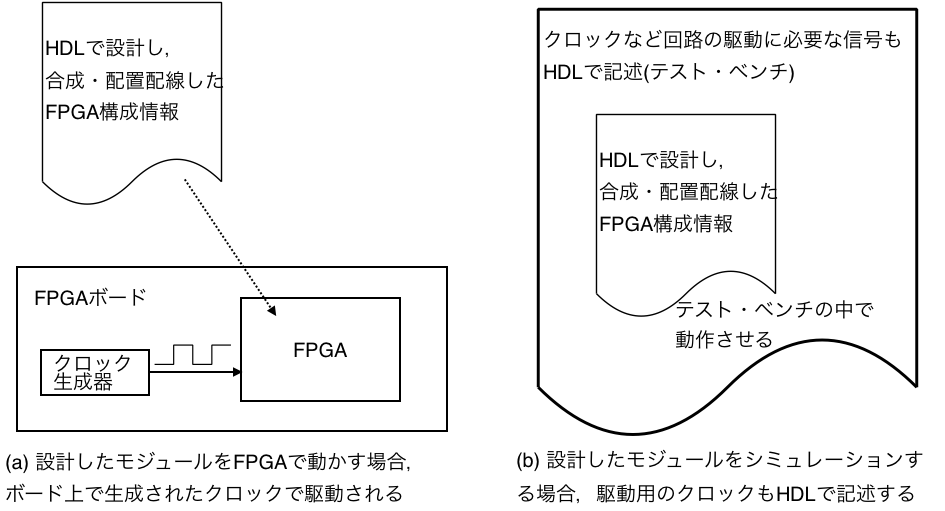
\includegraphics[width=.95\textwidth]{chapter04_figures/test_bench_image.png}
  \end{center}
  \caption{設計したモジュールを実機で動作させる場合(a)とシミュレーションする場合(b)の違い.シミュレーションする場合にはテスト・ベンチを用意する必要がある.\label{fig:test_bench_image}}
 \end{figure}

といっても,とりたてて新しく特別なことを覚える必要があるわけではありません.外から与えられるべきクロック信号やリセット信号もHDLで記述できます.これをシミュレーション・コードやテスト・ベンチと呼びます.シミュレーション対象のモジュールで必要となる信号は,すべてテスト・ベンチで生成します.テスト・ベンチの記述方法はHDLソースとほとんど同じで,違いは下記の3つになります.

\begin{itemize}
 \item エンティティの中身(モジュールの入出力信号)が空である 
 \item 時間を表す構文を使って信号の振る舞いを規定する 
 \item ハードウェアでは実現できない仮想的な機能を利用できる 
\end{itemize}

設計したHDLモジュールを動作させるのには必要な,マザーボードに相当する部分をすべて記述しなければなりません.逆にいうと,テスト・ベンチは外部との入出力があってはいけないということです.そのため,VHDLの場合はテスト・ベンチのエンティティの中身が,Verilog HDLの場合moduleの引数が空になるというわけです.

\subsection{テスト・ベンチでは``時間''を表現する必要がある}
「スイッチを10秒押してから離す」や「50MHzの信号」などの振る舞いは時間を扱うので,HDLのビヘイビア・モデル(動作記述)を用いて記述します.

たとえば,「10nsの時間を待つ」という動作はHDLで次のように記述します.この記述はビヘイビア・モデルの基本中の基本です.
VHDLで記述する場合は,
\begin{figure}[H]
\begin{quote}
\begin{Verbatim}[frame=single, numbers=left, baselinestretch=0.8]
wait for 10ns;
\end{Verbatim}
\end{quote}
\end{figure}
Verilog HDLで記述する場合には,初めに`timescaleを使って,
\begin{figure}[H]
\begin{quote}
\begin{Verbatim}[frame=single, numbers=left, baselinestretch=0.8]
`timescale 1ns / 1ps
\end{Verbatim}
\end{quote}
\end{figure}
と,シミュレーションの単位時間を指定して,時間を挿入したい個所で
\begin{figure}[H]
\begin{quote}
\begin{Verbatim}[frame=single, numbers=left, baselinestretch=0.8]
#10
\end{Verbatim}
\end{quote}
\end{figure}
と記述すると,指定した単位時間分の時間(この例では10ns)を作ることができます.

\section{テストベンチの書き方}
またか!!という感も否めませんが,「LEDチカチカ」に再び登場してもらいましょう.コードは次の通りです.前章で利用したコードといくつかの違いがあります.

\paragraph{resetの追加}
回路を初期化するための入力信号としてresetを追加しています.

\paragraph{LEDに出力するbitを変更}
実機ではカウンタの23bit目をledに接続しましたが,クロックの立ち上がりを8M回待つのは大変なので3bit目をledの出力に接続しています.

\paragraph{モジュールのタイプをRTLに変更}
モジュールのタイプをBehaviorではなくRTLとしています.実際のところ今のVivadoでは,ここのキーワードは特に意味をなさないのですがシミュレーションのためのテストベンチをBehavior,合成してハードウェア化もするファイルはRTLと分けておくと見分けるのが容易になります.

\begin{figure}[H]
\begin{quote}
\begin{Verbatim}[frame=single, numbers=left, baselinestretch=0.8]
 library ieee;
 use ieee.std_logic_1164.all;
 use ieee.numeric_std.all;

 entity top is
    Port ( clk   : in std_logic;
           reset : in std_logic;
           led   : out std_logic
         );
 end top;

 architecture RTL of top is

  signal counter : unsigned(31 downto 0) := (others => '0');

 begin

  -- カウンタの3bit目をledに接続(実機では23bit目を使った)
  led <= std_logic(counter(3));

  process(clk) -- クロックの変化で動作するプロセス
  begin
    if rising_edge(clk) then -- クロックの立ち上がりであれば
      if reset = '1' then
        counter <= (others => '0');
      else
        counter <= counter + 1; -- カウンタをインクリメント
      end if;
    end if;
  end process;

 end RTL;
\end{Verbatim}
\end{quote}
\caption{シミュレーション対象のコード\label{fig:target_list}}
\end{figure}

FPGA上に実装する場合には,第3章で紹介したように,3つの入出力信号をFPGA上の適切なI/Oに接続しなければなりません.一方,ソフトウェアで動作をシミュレーションするためには,これらの信号テスト・ベンチで生成して外から与える,ことにします.

\subsection{クロックを生成するテスト・ベンチ}
順序回路の要がクロック信号です.従って,クロック信号の生成はテスト・ベンチの基本中の基本です.

カウンタ・モジュールの動作をシミュレーションするために,
\verb|clk|に50MHzのクロック信号,すなわち10nsごとに\verb|‘1’|と\verb|‘0’|を繰り返す信号をテスト・ベンチで生成してみましょう.
記述方法は,次の通りです.

\subsubsection{VHDLで記述する場合}

信号\verb|clk_i|を定義し,\verb|clk_i|に‘1’を代入して10ns待ちます.その10ns後\verb|clk_i|に‘0’を代入,その10n後に再び‘1’を\verb|clk_i|に代入,…ということを繰り返すことで,10nsで周期的に0→1→0→1...と変化する信号,すなわち50MHzのクロック信号が生成できます.
VHDLのコードで素直に実装すると,「10ns待つ」処理に相当する「wait for 10ns」を使って,
\begin{figure}[H]
\begin{quote}
\begin{Verbatim}[frame=single, numbers=left, baselinestretch=0.8]
process begin
  clk_i <= '1';
  wait for 10ns;
  clk_i <= '0';
  wait for 10ns;
  clk_i <= '1';
  wait for 10ns;
  clk_i <= '0';
  wait for 10ns;
  ...
end process;
\end{Verbatim}
\end{quote}
\end{figure}
となります.

この\verb|process|文には,きっかけになる信号なしで,シミュレーションの開始同時にすぐさま処理が開始されます.
もちろん,これでもよいのですが,実はプロセス文は最後まで到達すると,また先頭から開始されるので
\begin{figure}[H]
\begin{quote}
\begin{Verbatim}[frame=single, numbers=left, baselinestretch=0.8]
process begin
  clk_i <= '1'; wait for 10ns;
  clk_i <= '0'; wait for 10ns;
end process;
\end{Verbatim}
\end{quote}
\end{figure}
という記述で,ずっとクロック信号を作り続けることができます.

\subsubsection{Verilog HDLで記述する場合}
Verilog HDLでは,「単位時間XXが経過」を「\verb|#XX|」で表現できますから,\verb|clk_i|に'1'を代入したあと,
「単位時間10が経過」の後\verb|clk_i|に'0'を代入して,また「単位時間10が経過」の後\verb|clk_i|に'1'を代入...
と繰り返すことで,1→0→1→...というシーケンスが定義できます.

Verilog HDLでは,initial文で,シミュレーション実行開始時に一度だけ処理されるブロックを定義できます.
すなわち,次のコード片で,シミュレーション開始後から単位時間10毎に信号を反転させる処理,つまり50MHzのクロック信号を生成できます.
\begin{figure}[H]
\begin{quote}
\begin{Verbatim}[frame=single, numbers=left, baselinestretch=0.8]
initial begin
  clk_i = 0; #10;
  clk_i = 1; #10;
  ...
  forever #10 clk_i = !clk_i;
end
\end{Verbatim}
\end{quote}
\end{figure}

ずっと繰り返す処理を意味する\verb|forever|を使って,
\begin{figure}[H]
\begin{quote}
\begin{Verbatim}[frame=single, numbers=left, baselinestretch=0.8]
initial begin
  clk_i = 0;
  forever #10 clk_i = !clk_i;
end
\end{Verbatim}
\end{quote}
\end{figure}
と記述することもできます.

\subsection{必要な入力信号を生成する}

図\ref{fig:target_list}に示したリストの動作をシミュレーションするにはクロック信号clk以外に,人間が「えいやっ」とリセット・ボタンを押すことに相当するreset信号もテスト・ベンチで生成しなければいけません.

ところで,人間がリセット・ボタンを押すのは,いつ,どのくらいの時間でしょうか?「リセット・ボタンは電源投入の5秒後に10ミリ秒間押される」などと決められるわけではありません.

従って,テスト・ベンチでは,シミュレーション対象の回路に対して,それらしい信号を想定して生成する必要があります.リセット・ボタンが押されるタイミング,であれば,特に制約があるわけではありませんので,電源投入後の適当な時刻に検知できる時間だけの信号が与えられる,という想定で十分でしょう.

リセット信号を生成する方法は,
\begin{enumerate}
 \item クロックと同じプロセス・ブロックで記述する
 \item 別のプロセスのブロック内で記述する
\end{enumerate}
の2種類が考えられます.

ここでは,クロックとは別のプロセス・ブロック内で,変数\verb|reset_i|の値を0→1→0と変化させることで,リセット・ボタンが押されたことに相当する信号を生成することにします.Verilog HDLであれば,リセットに相当するレジスタ変数\verb|reset_i|が適当なタイミングで変化するように記述できます.
\begin{figure}[H]
\begin{quote}
\begin{Verbatim}[frame=single, numbers=left, baselinestretch=0.8]
initial begin
  reset_i <= '0'; -- 最初はリセット信号は'0'
  wait for 5ns;
  reset_i <= '1'; -- 5n秒後にリセット信号を'1'に
  wait for 100ns;
  reset_i <= '0'; -- しばらくしたら(100n秒後),リセット信号を'0'に
  wait; -- 以降は何もしない
end
\end{Verbatim}
\end{quote}
\end{figure}

\subsection{テスト・ベンチとシミュレーション対象のモジュールを接続する}
FPGA上に書き込んだ回路に信号を与えるためには,物理的にクロックやスイッチの端子を配線することになります.
シミュレーションする場合には,シミュレーション対象のモジュールとテスト・ベンチで生成した信号をHDL的に接続する必要があります.

一般的には,テスト・ベンチをトップ・モジュールとして,
その中でカウンタ・モジュールをサブモジュールとして呼び出すことにします.
これはマザー・ボードがあって,その中にFPGAがあって回路が動いている,という物理的な構造に上手くマッチします.
VHDLもVerilog HDLも,モジュールを階層的に定義する仕組みをもっています.

VHDLでは,
\begin{enumerate}
 \item LEDチカチカ回路のインターフェースを宣言
 \item LEDチカチカ回路のインスタンスを生成する
\end{enumerate}
の2段階で,サブモジュールとして回路を呼び出すことができます.

具体的には,はじめに,次のように,
\begin{figure}[H]
\begin{quote}
\begin{Verbatim}[frame=single, numbers=left, baselinestretch=0.8]
-- サブ・モジュールであるtestの素性を記述
component test
  port (
    clk   : in std_logic;
    reset : in std_logic;
    led   : out std_logic
);
end component;
\end{Verbatim}
\end{quote}
\end{figure}
\verb|component|として,使用するモジュールの素性を宣言したあとで,次のように
\begin{figure}[H]
\begin{quote}
\begin{Verbatim}[frame=single, numbers=left, baselinestretch=0.8]
-- サブ・モジュールをインスタンス化する
U: test port map(
     clk   => clk_i,
     reset => reset_i
     led   => led,
   );
\end{Verbatim}
\end{quote}
\end{figure}
このモジュールのインスタンスを生成,配線関係を記述します.

プログラミング言語Cでも,関数を呼び出す時には,関数の素性を明らかにするために「プロトタイプ宣言」をした上で,
関数呼び出し文を書きますよね.VHDLでも同じようなものだな,と考えてもらえればよいでしょう.

\subsection{テスト・ベンチの全容}

説明が長くなりましたが,図\ref{fig:target_list}のリストをシミュレーションするためのテスト・ベンチの全容は,
図\ref{fig:simulation_list}のようになります.

\begin{figure}[H]
\begin{quote}
\begin{Verbatim}[frame=single, numbers=left, baselinestretch=0.8]
library ieee;
use ieee.std_logic_1164.all;
use ieee.numeric_std.all;
entity top_sim is
end top_sim;
architecture Behavioral of top_sim is
  -- シミュレーション対象のモジュールを宣言
  component top
    Port ( clk   : in std_logic;
           reset : in std_logic;
           led   : out std_logic
           );
  end top;
  -- シミュレーション対象のモジュールの信号用の変数を宣言
  signal clk_i   : std_logic := '0';
  signal reset_i : std_logic := '0';
  signal led_i   : std_logic := '0';
begin
  -- シミュレーション対象のモジュールのインスタンス生成
  U : top port map(
    clk => clk_i,
    reset => reset_i,
    led => led_i
    );
  -- クロックを生成
  process
  begin
    clk_i <= '1'; wait for 10ns;
    clk_i <= '0'; wait for 10ns;
  end process;
  -- リセット信号の生成
  process
  begin
    reset_i <= '0';
    wait for 5ns;
    reset_i <= '1';
    wait for 100ns;
    reset_i <= '0';
    wait;
  end process;
end Behavioral;
\end{Verbatim}
\end{quote}
\caption{図\ref{fig:target_list}をシミレーションするためのVHDLによるテスト・ベンチ\label{fig:simulation_list}}
\end{figure}

\section{シミュレーションの実行手順}

シミュレーションのテスト用に新しくプロジェクトを作成しましょう.
プロジェクト名は,\verb|project_2|としました.

 \begin{figure}[H]
  \begin{center}
   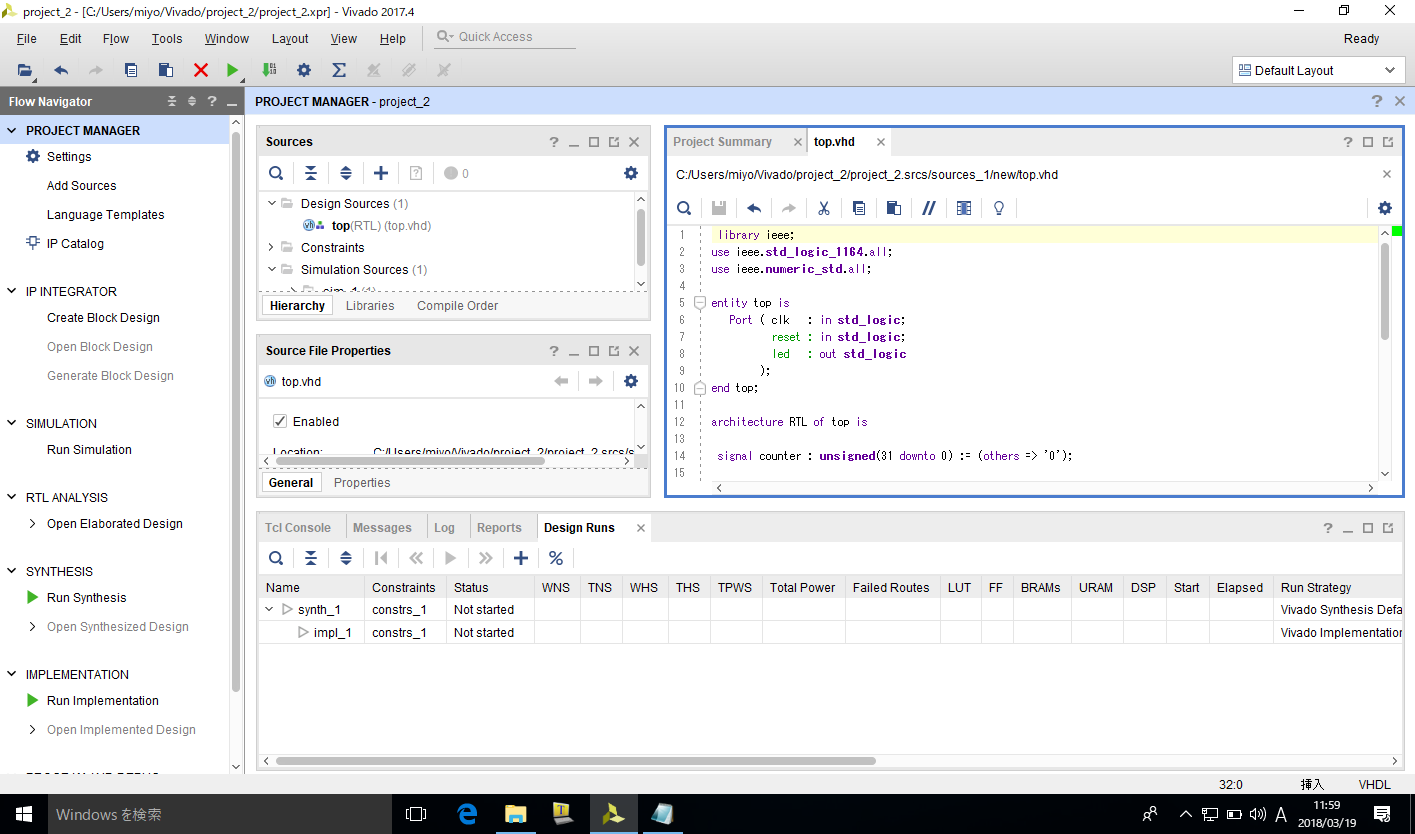
\includegraphics[width=.8\textwidth]{chapter04_figures/VirtualBox_Windows10_19_03_2018_11_59_40.png}
  \end{center}
  \caption{新しく作成したプロジェクト}
 \end{figure}

前章と同様にtopモジュールを作成・追加してプロジェクトを作成したら,
topモジュールの中身を図\ref{fig:target_list}のように変更しておきます.

以降の手順は次の通りです.

 \begin{figure}[H]
  \begin{center}
   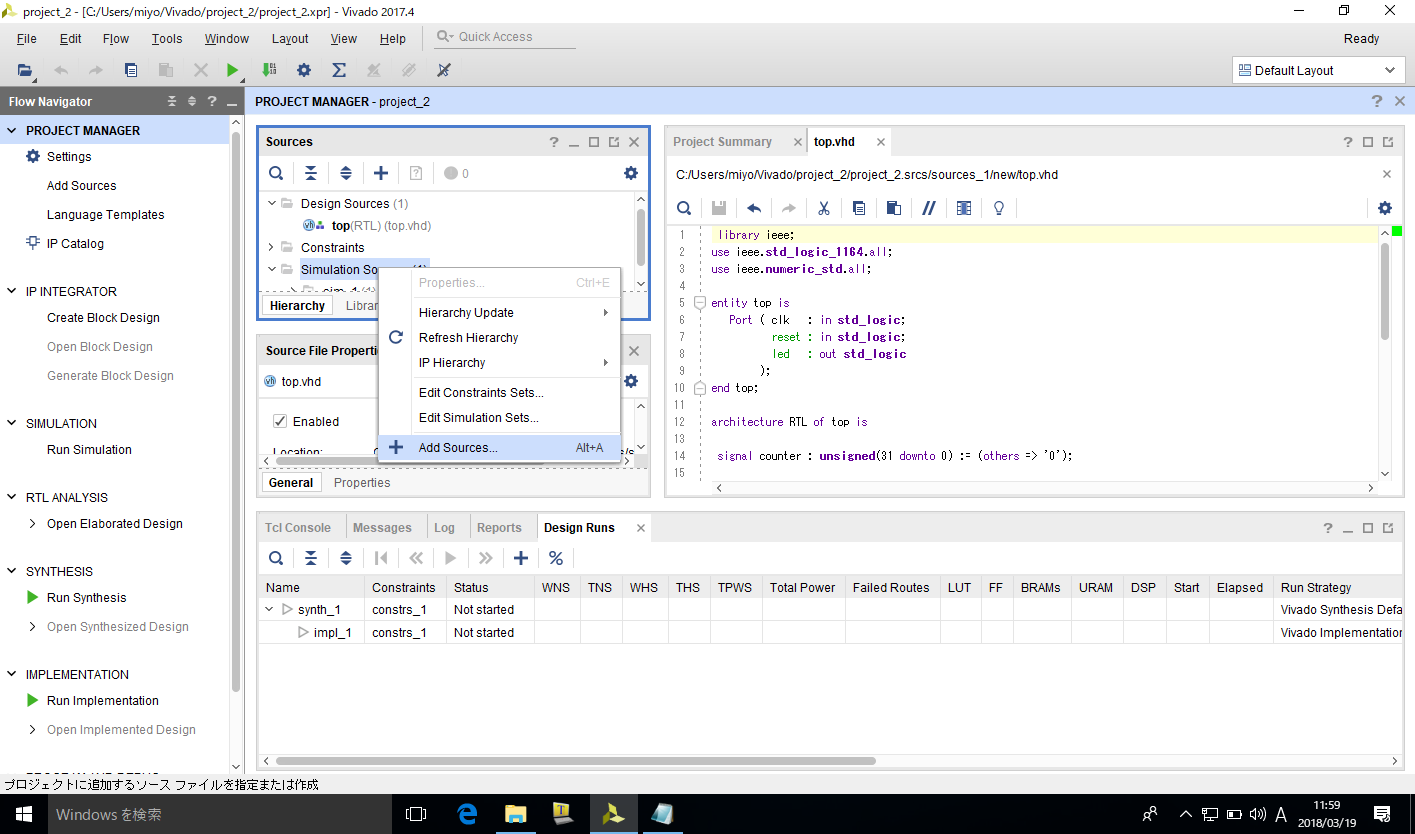
\includegraphics[width=.8\textwidth]{chapter04_figures/VirtualBox_Windows10_19_03_2018_11_59_46.png}
  \end{center}
  \caption{Sourcesの中のSimulation Sourcesの上で右クリックしてAdd Sourcesを選択}
 \end{figure}

 \begin{figure}[H]
  \begin{center}
   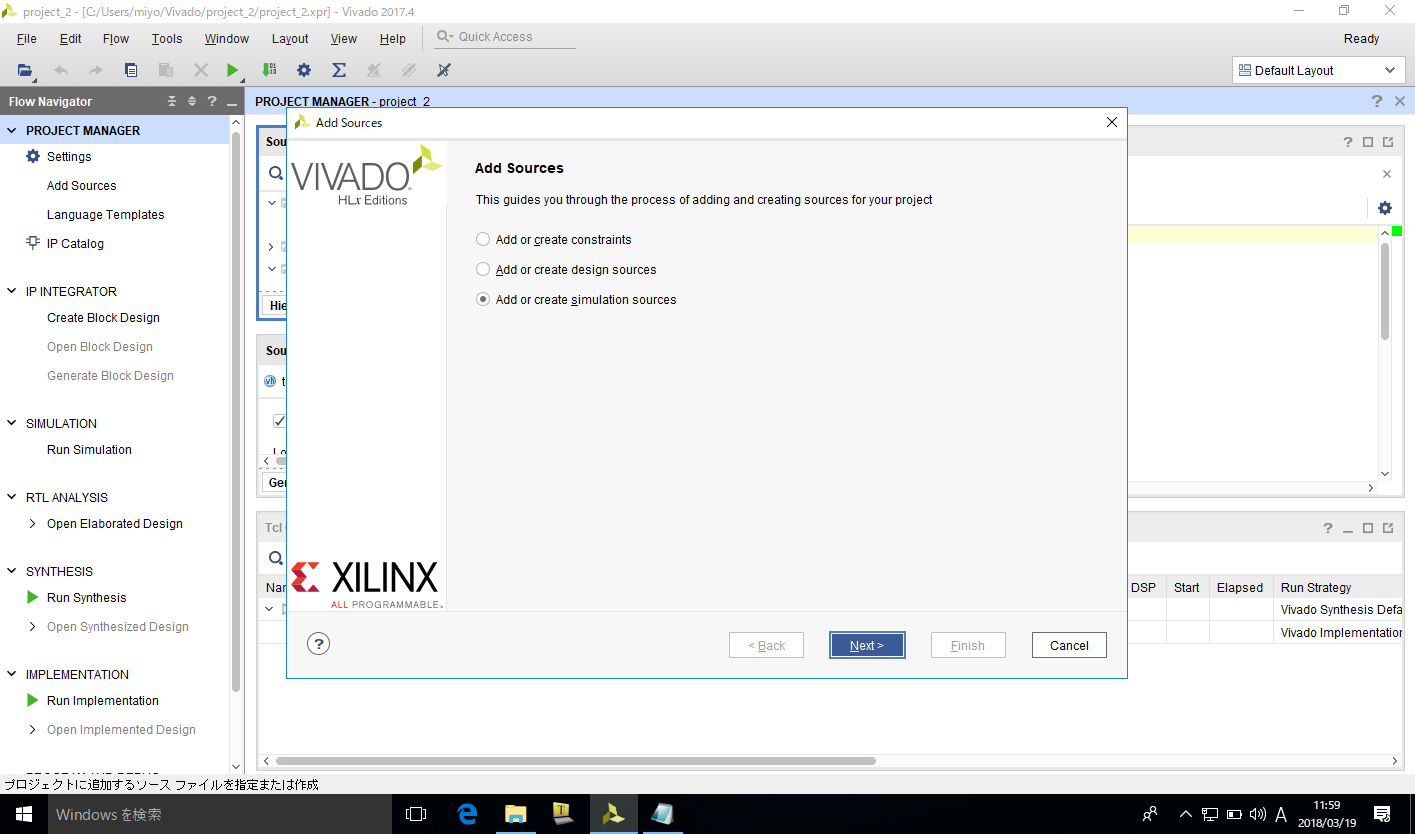
\includegraphics[width=.8\textwidth]{chapter04_figures/VirtualBox_Windows10_19_03_2018_11_59_52.png}
  \end{center}
  \caption{``Add or create simulation sources''にチェックが入っていることを確認してNextをクリック}
 \end{figure}

 \begin{figure}[H]
  \begin{center}
   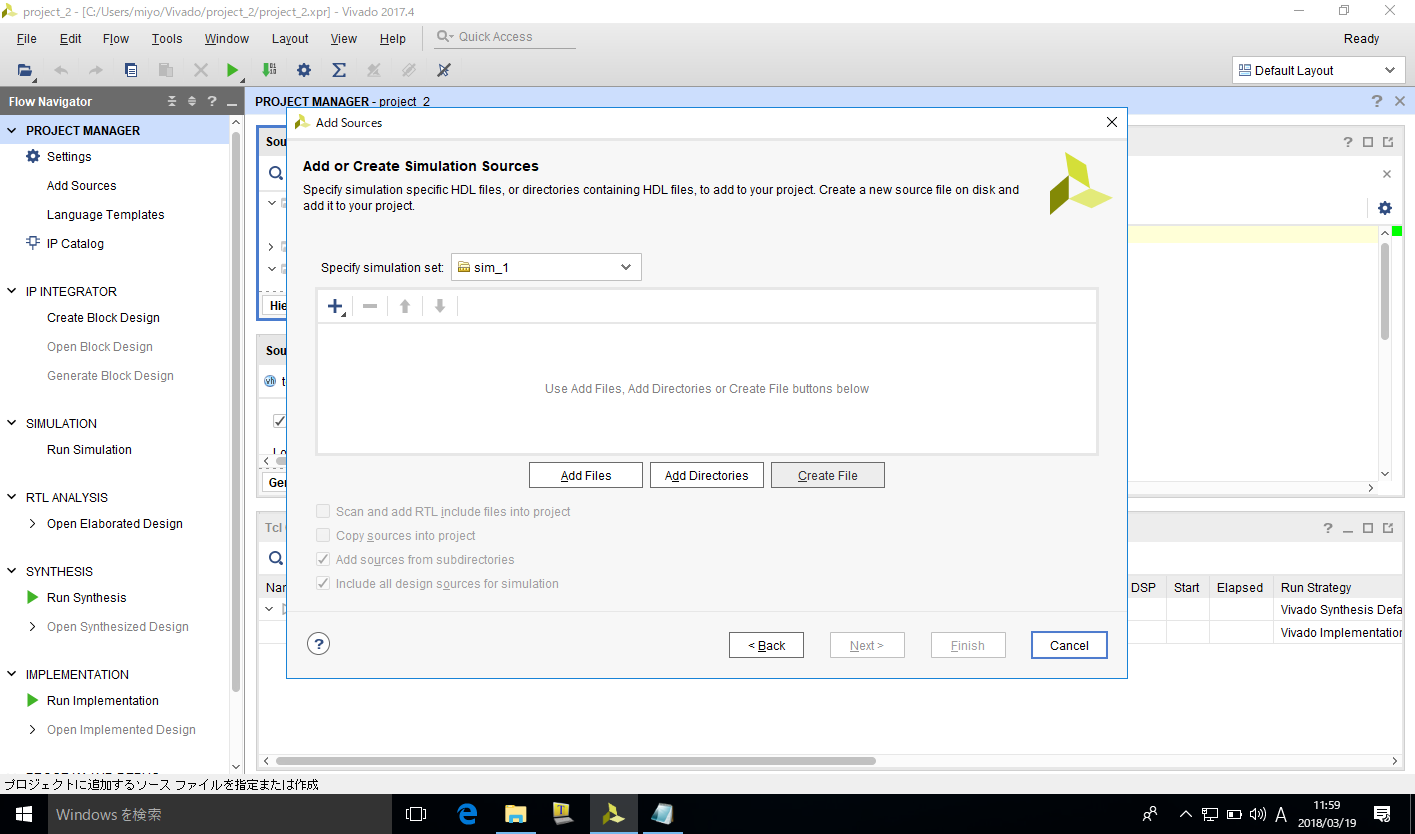
\includegraphics[width=.8\textwidth]{chapter04_figures/VirtualBox_Windows10_19_03_2018_12_00_00.png}
  \end{center}
  \caption{ファイル追加ダイアログで,Create Fileを選択}
 \end{figure}

 \begin{figure}[H]
  \begin{center}
   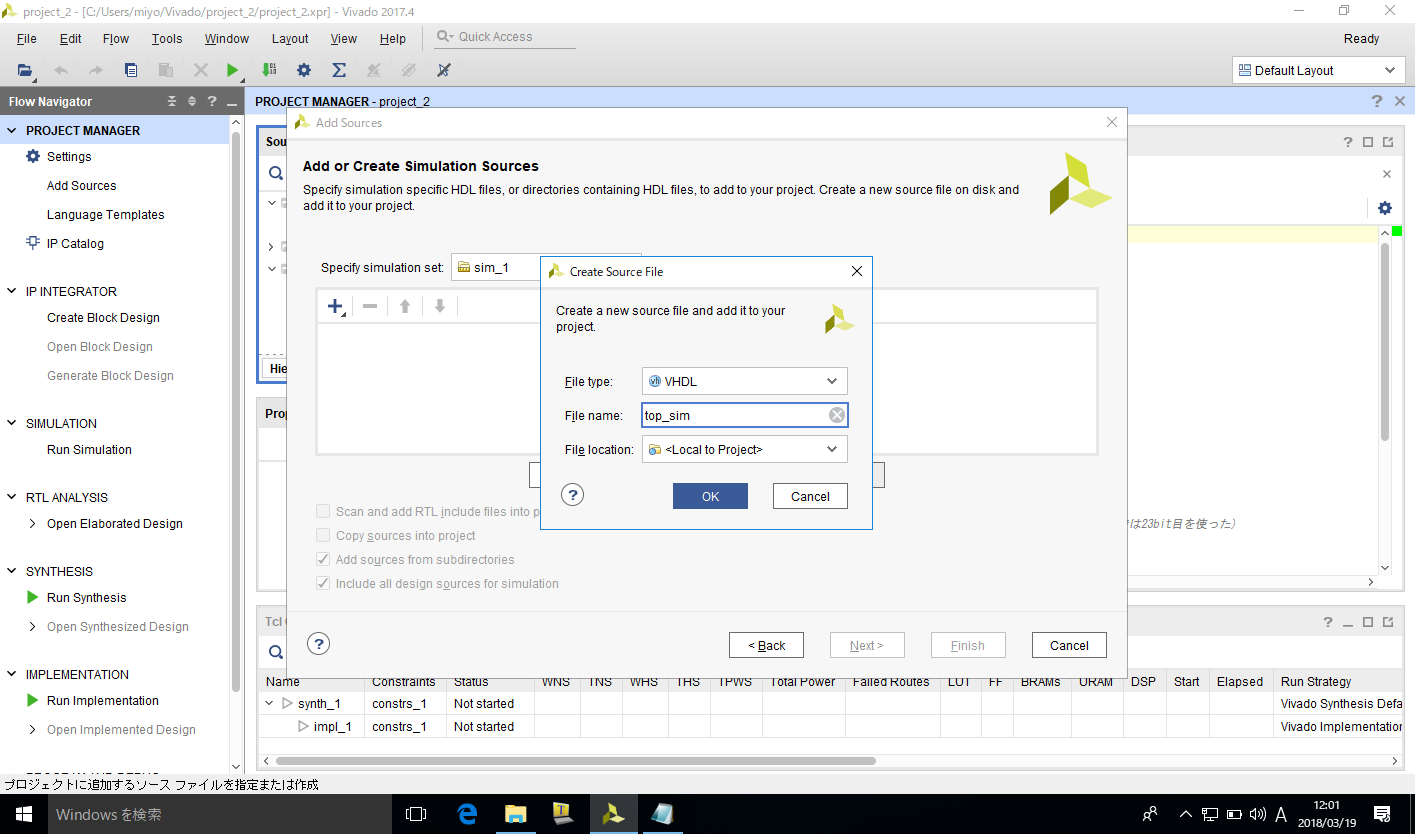
\includegraphics[width=.8\textwidth]{chapter04_figures/VirtualBox_Windows10_19_03_2018_12_01_34.png}
  \end{center}
  \caption{VHDLファイルとして,top\_simという名前のモジュールを作成する}
 \end{figure}

 \begin{figure}[H]
  \begin{center}
   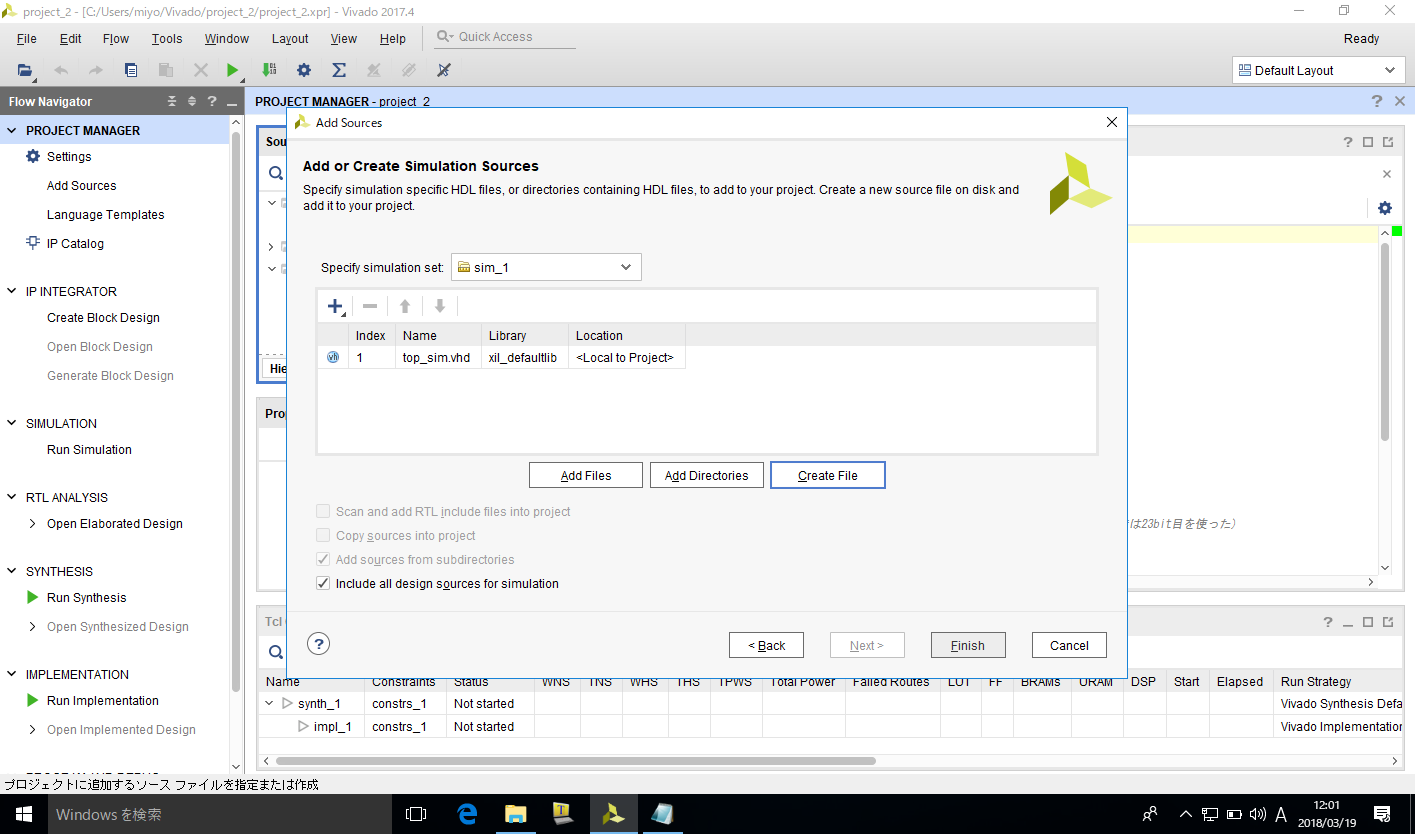
\includegraphics[width=.8\textwidth]{chapter04_figures/VirtualBox_Windows10_19_03_2018_12_01_42.png}
  \end{center}
  \caption{リストに追加された}
 \end{figure}

 \begin{figure}[H]
  \begin{center}
   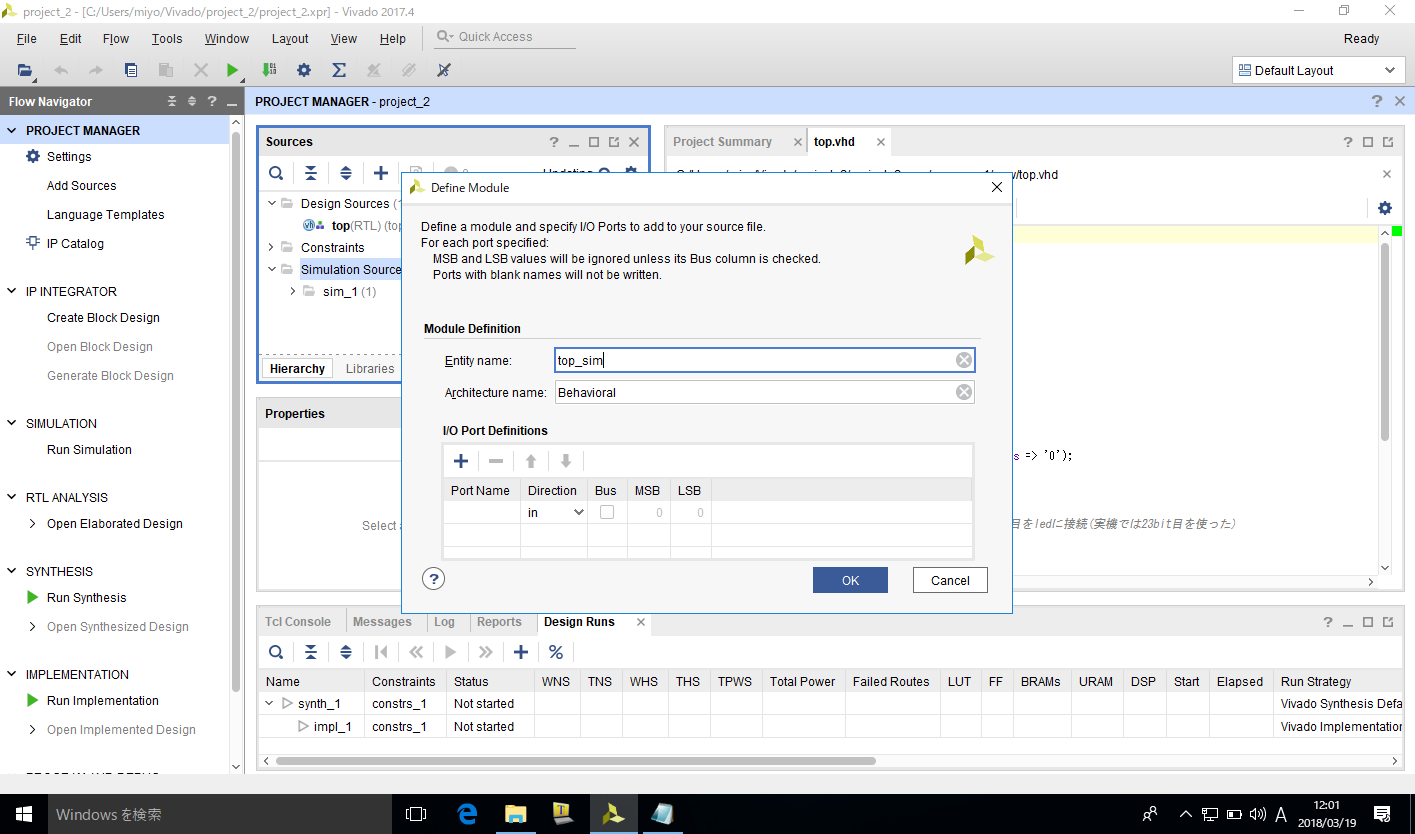
\includegraphics[width=.8\textwidth]{chapter04_figures/VirtualBox_Windows10_19_03_2018_12_01_49.png}
  \end{center}
  \caption{ポートの指定ダイアログ.今回は何もせずにOKをクリック}
 \end{figure}

 \begin{figure}[H]
  \begin{center}
   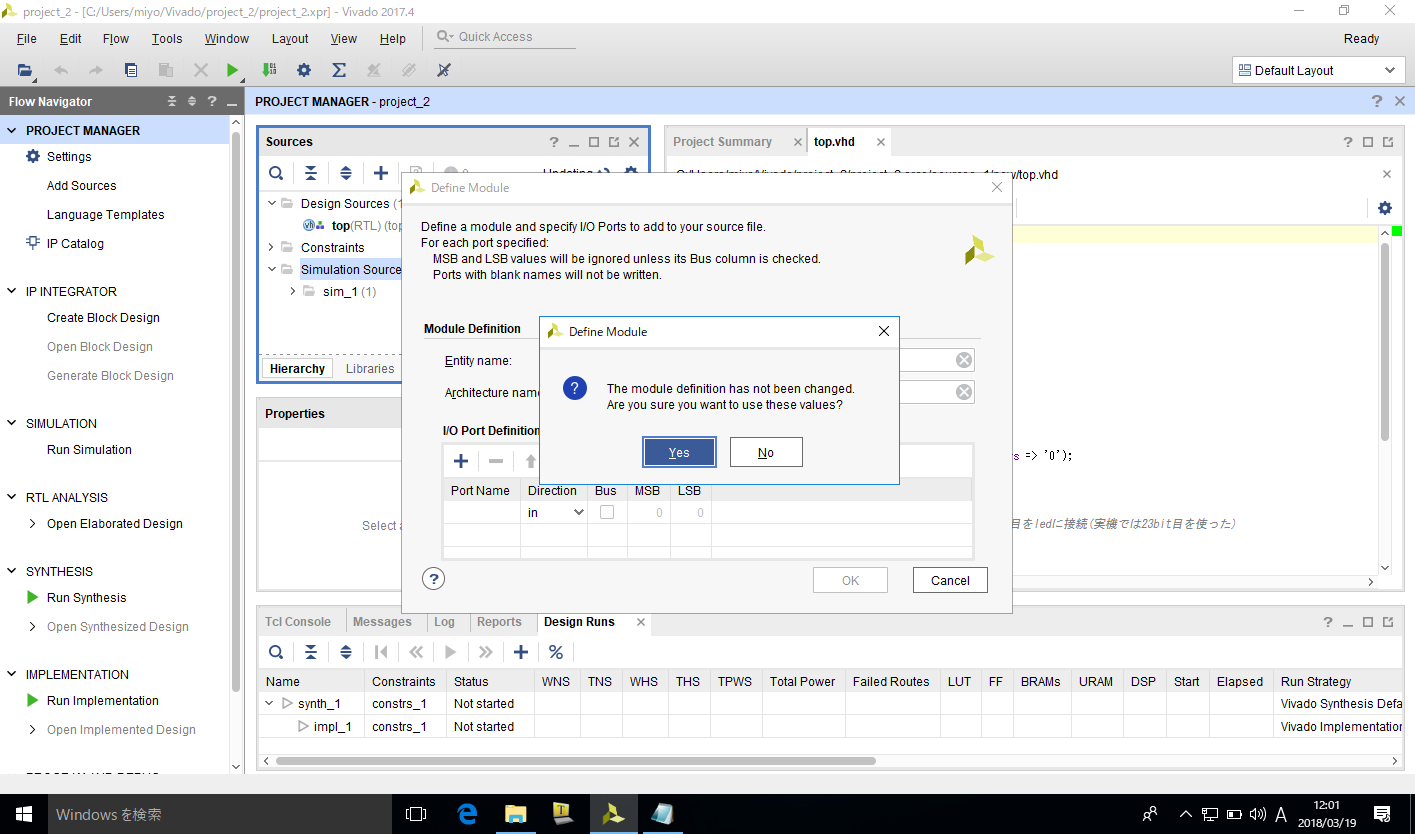
\includegraphics[width=.8\textwidth]{chapter04_figures/VirtualBox_Windows10_19_03_2018_12_01_54.png}
  \end{center}
  \caption{変更ないことを確認されるのでYesをクリックして,作業ステップをすすめる}
 \end{figure}

 \begin{figure}[H]
  \begin{center}
   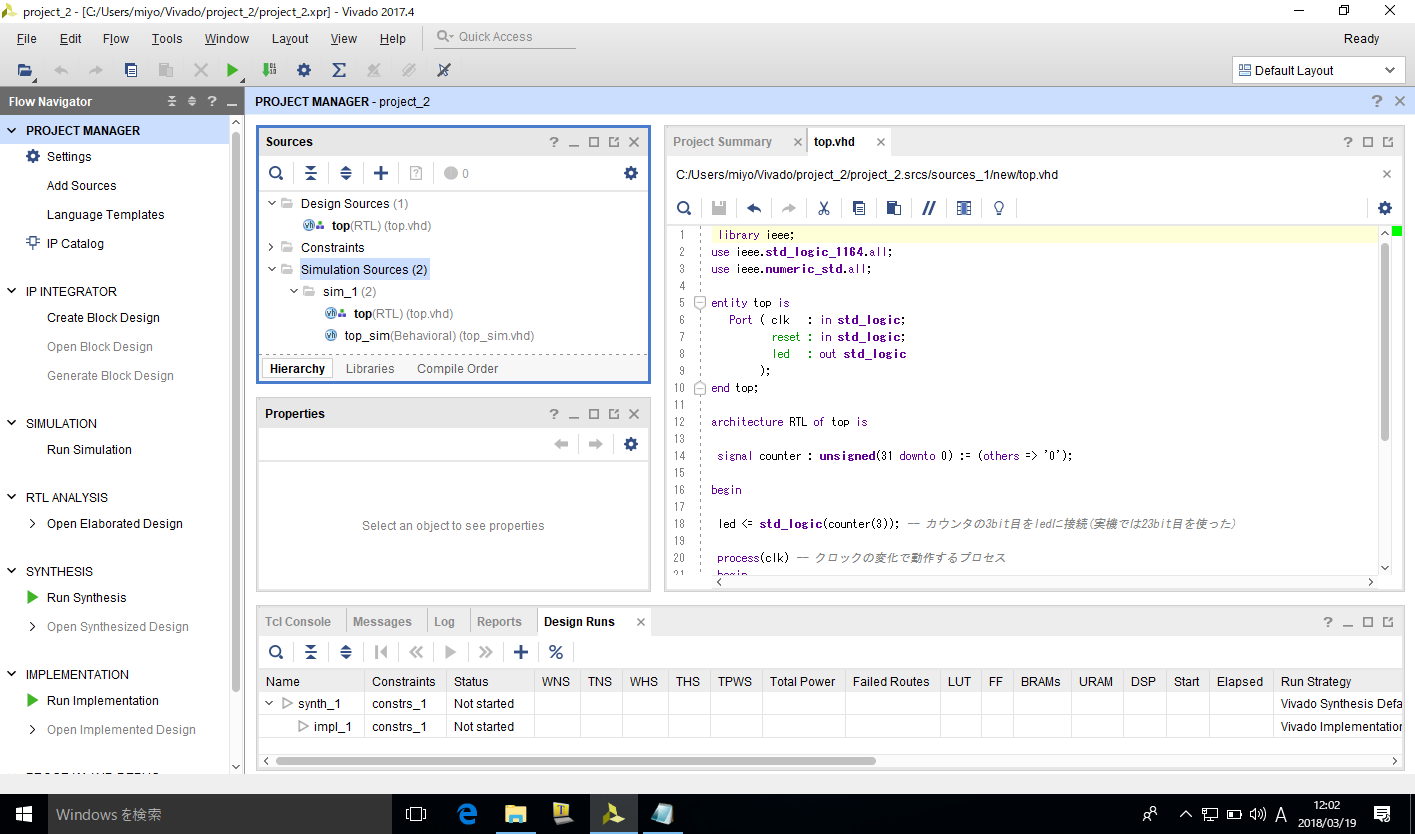
\includegraphics[width=.8\textwidth]{chapter04_figures/VirtualBox_Windows10_19_03_2018_12_02_05.png}
  \end{center}
  \caption{シミュレーション用のモジュールがプロジェクトに追加された}
 \end{figure}

 \begin{figure}[H]
  \begin{center}
   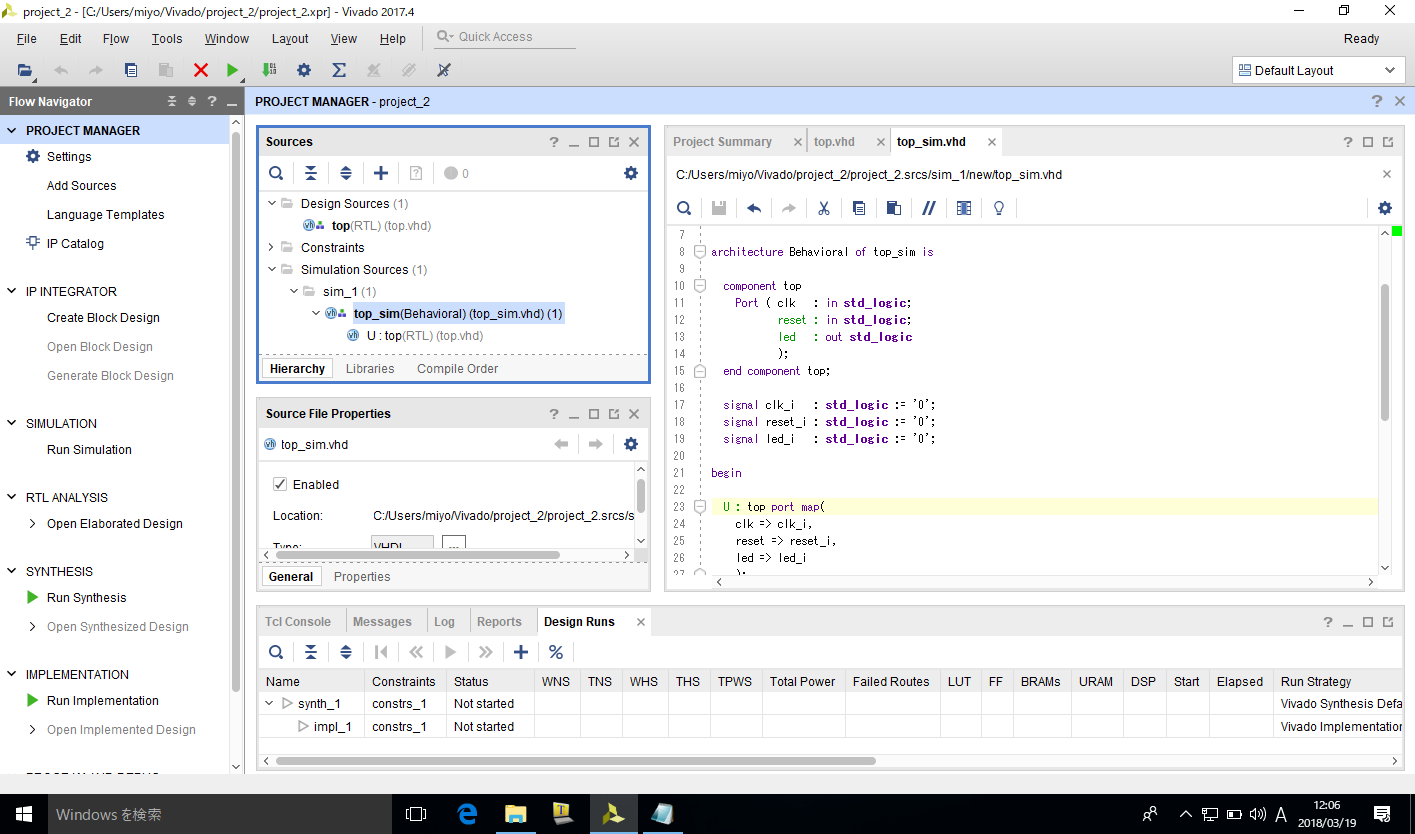
\includegraphics[width=.8\textwidth]{chapter04_figures/VirtualBox_Windows10_19_03_2018_12_06_25.png}
  \end{center}
  \caption{シミュレーションコードをtop\_simに反映したところ.top\_simからtopのモジュールがUという名前でインスタンス化されている様子が階層化されて表示される.}
 \end{figure}

 \begin{figure}[H]
  \begin{center}
   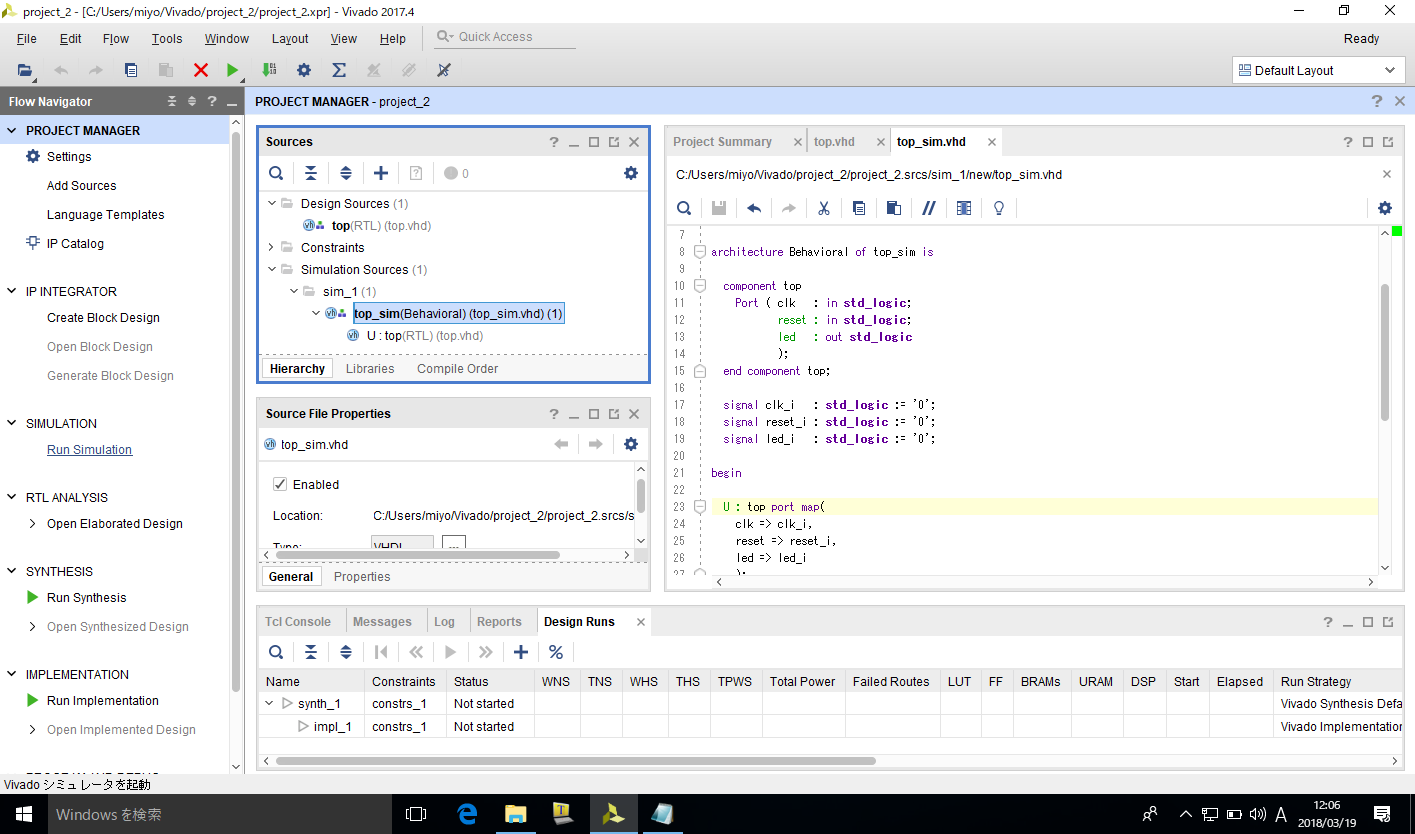
\includegraphics[width=.8\textwidth]{chapter04_figures/VirtualBox_Windows10_19_03_2018_12_06_33.png}
  \end{center}
  \caption{Flow NavigatorのRun Simulationでシミュレーションの開始}
 \end{figure}

 \begin{figure}[H]
  \begin{center}
   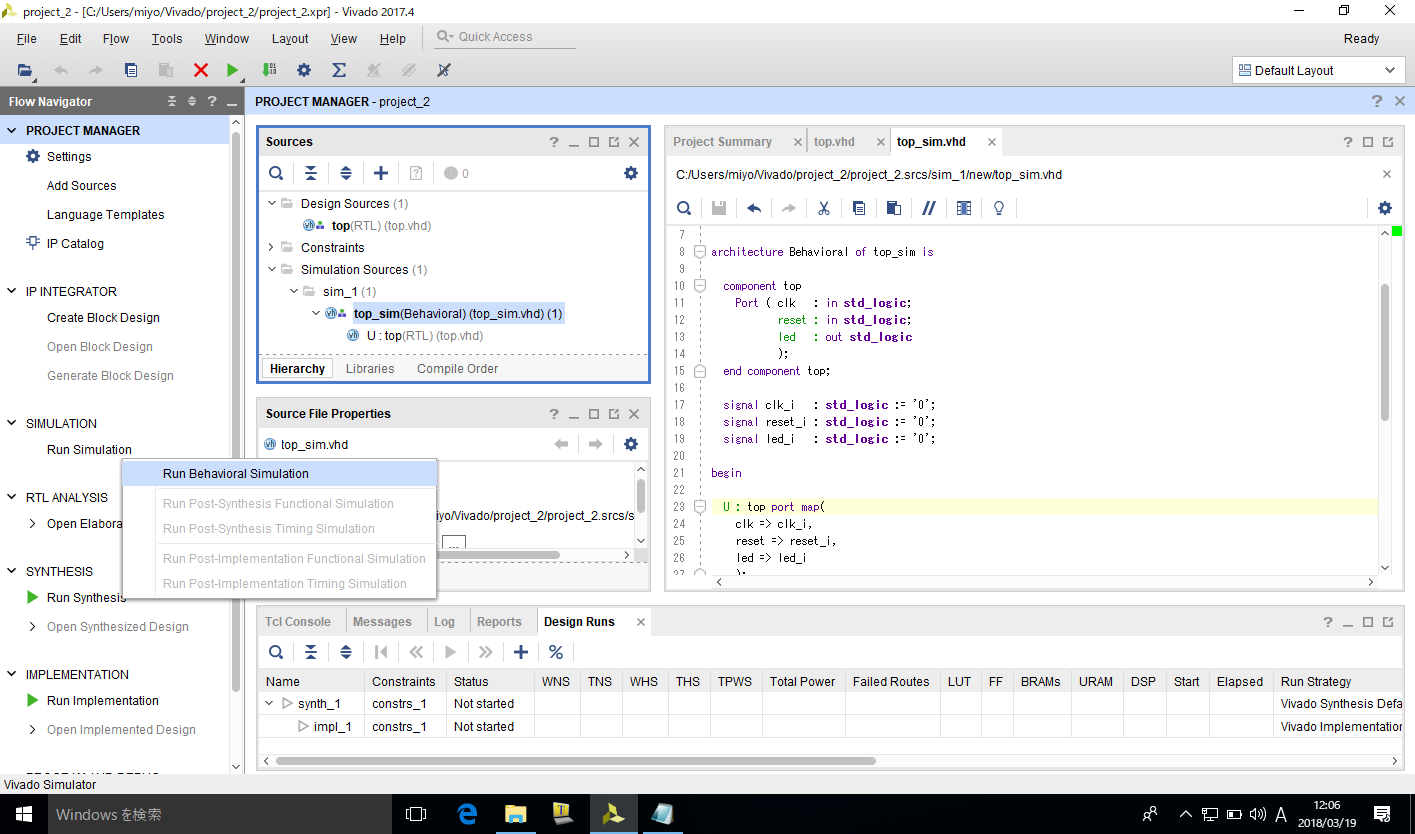
\includegraphics[width=.8\textwidth]{chapter04_figures/VirtualBox_Windows10_19_03_2018_12_06_40.png}
  \end{center}
  \caption{Run Behavioral Simultaionを選択}
 \end{figure}

 \begin{figure}[H]
  \begin{center}
   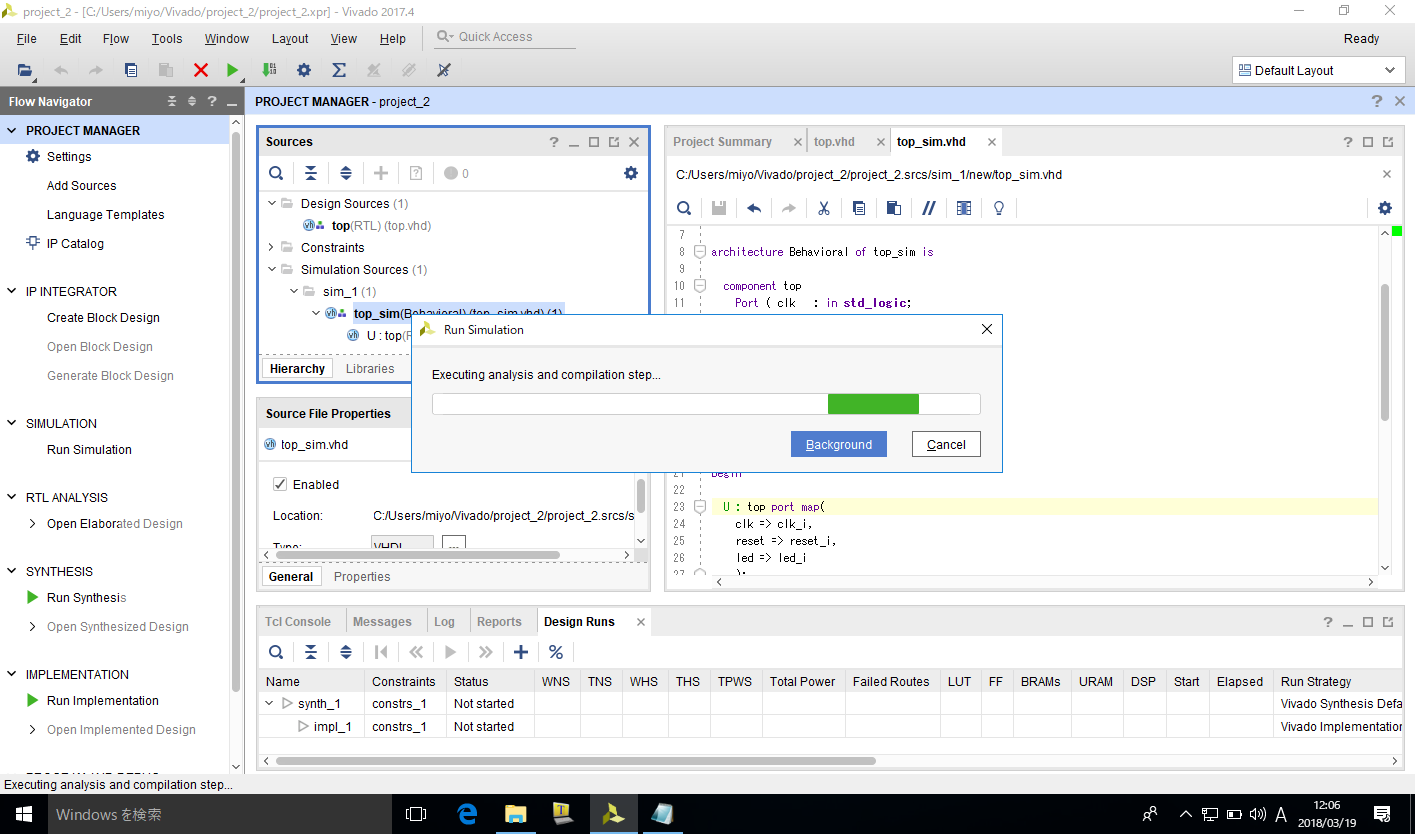
\includegraphics[width=.8\textwidth]{chapter04_figures/VirtualBox_Windows10_19_03_2018_12_06_45.png}
  \end{center}
  \caption{シミュレーション開始には少し時間がかかる}
 \end{figure}

 \begin{figure}[H]
  \begin{center}
   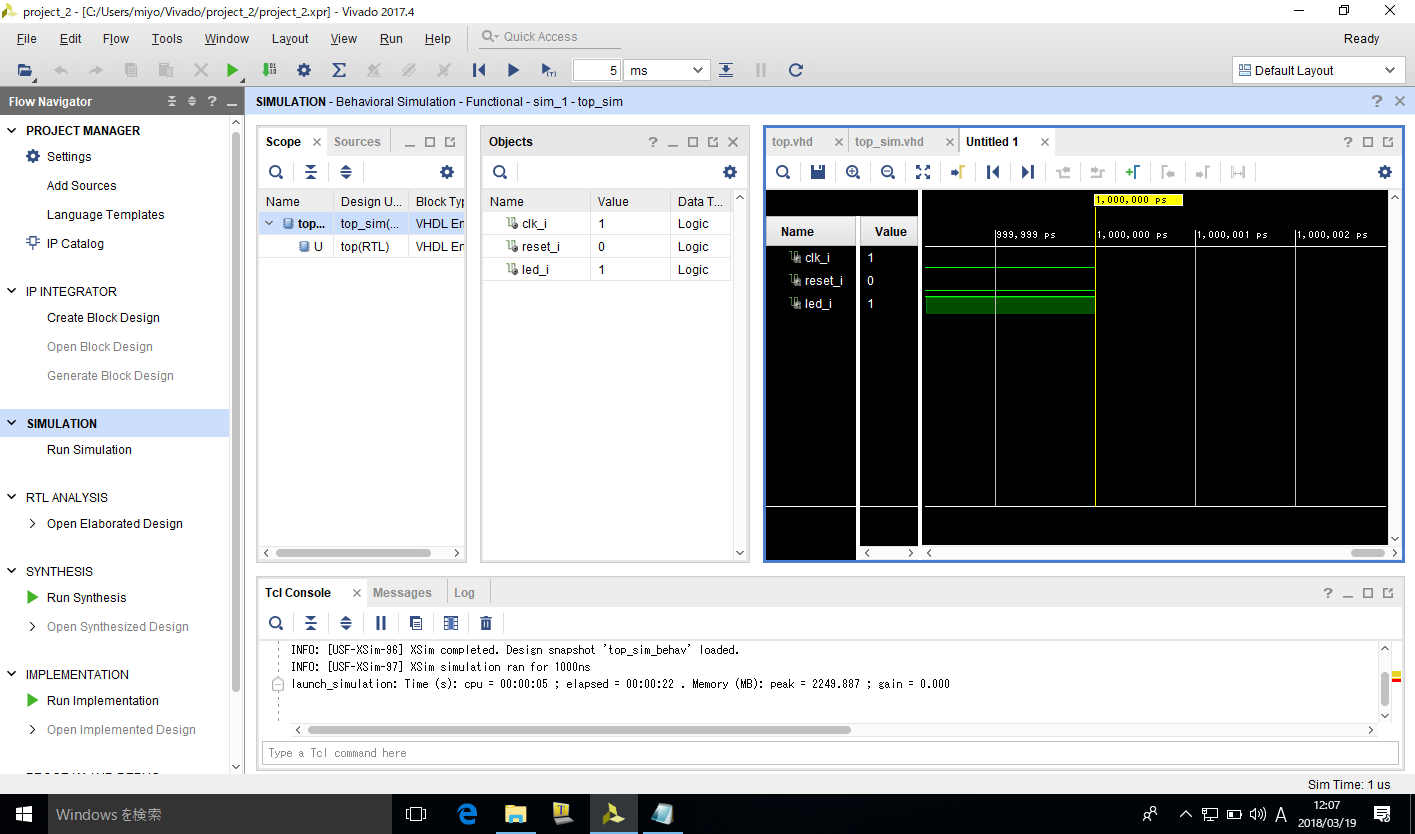
\includegraphics[width=.8\textwidth]{chapter04_figures/VirtualBox_Windows10_19_03_2018_12_07_37.png}
  \end{center}
  \caption{シミュレーションが開始された}
 \end{figure}

 \begin{figure}[H]
  \begin{center}
   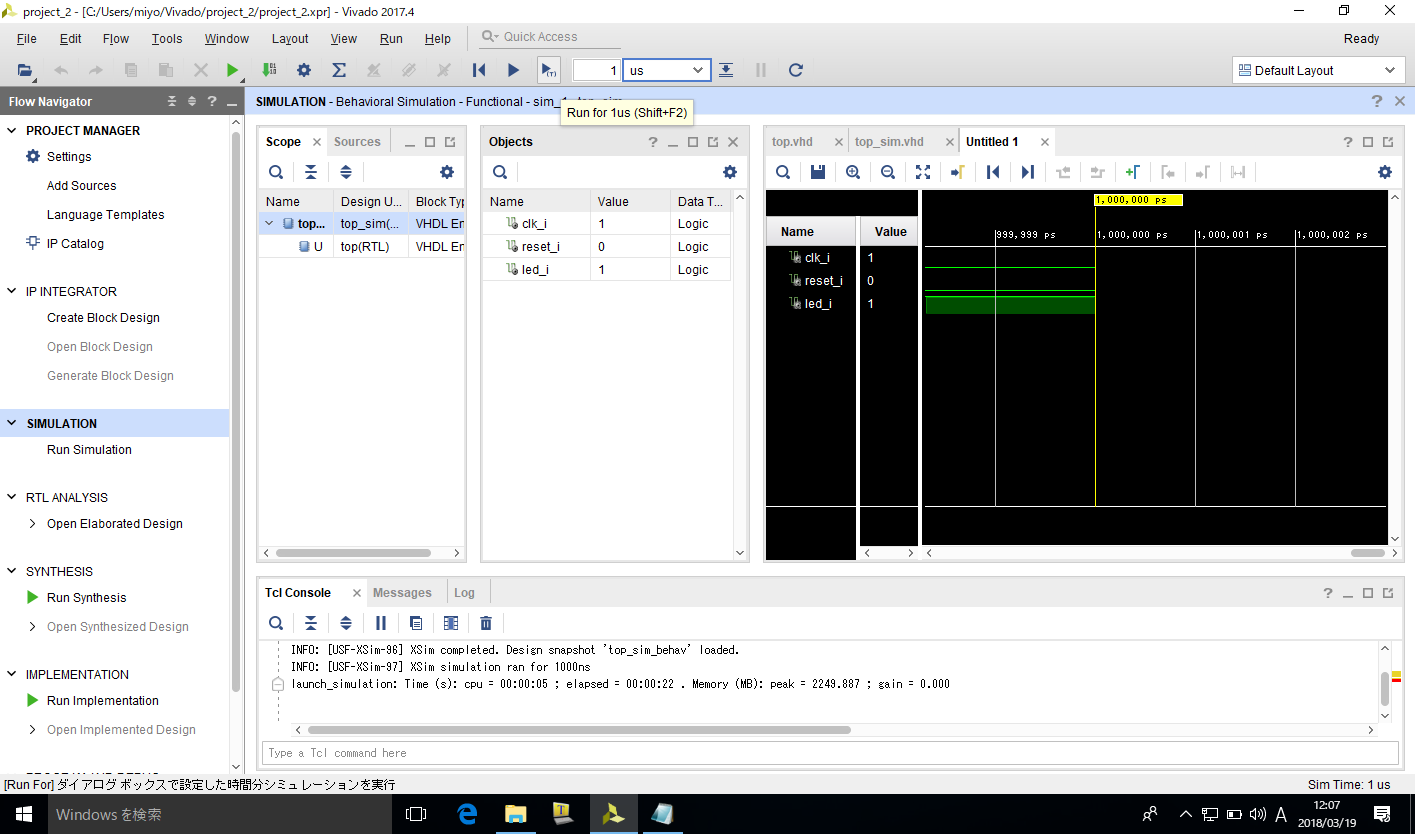
\includegraphics[width=.8\textwidth]{chapter04_figures/VirtualBox_Windows10_19_03_2018_12_07_58.png}
  \end{center}
  \caption{シミュレーション時間を指定して,シミュレーションステップをすすめる}
 \end{figure}

指定した時間のシミュレーションが終わるとストップします.いつまでもストップしない場合には,一時停止アイコンをクリックして,強制的に止めることができます.

 \begin{figure}[H]
  \begin{center}
   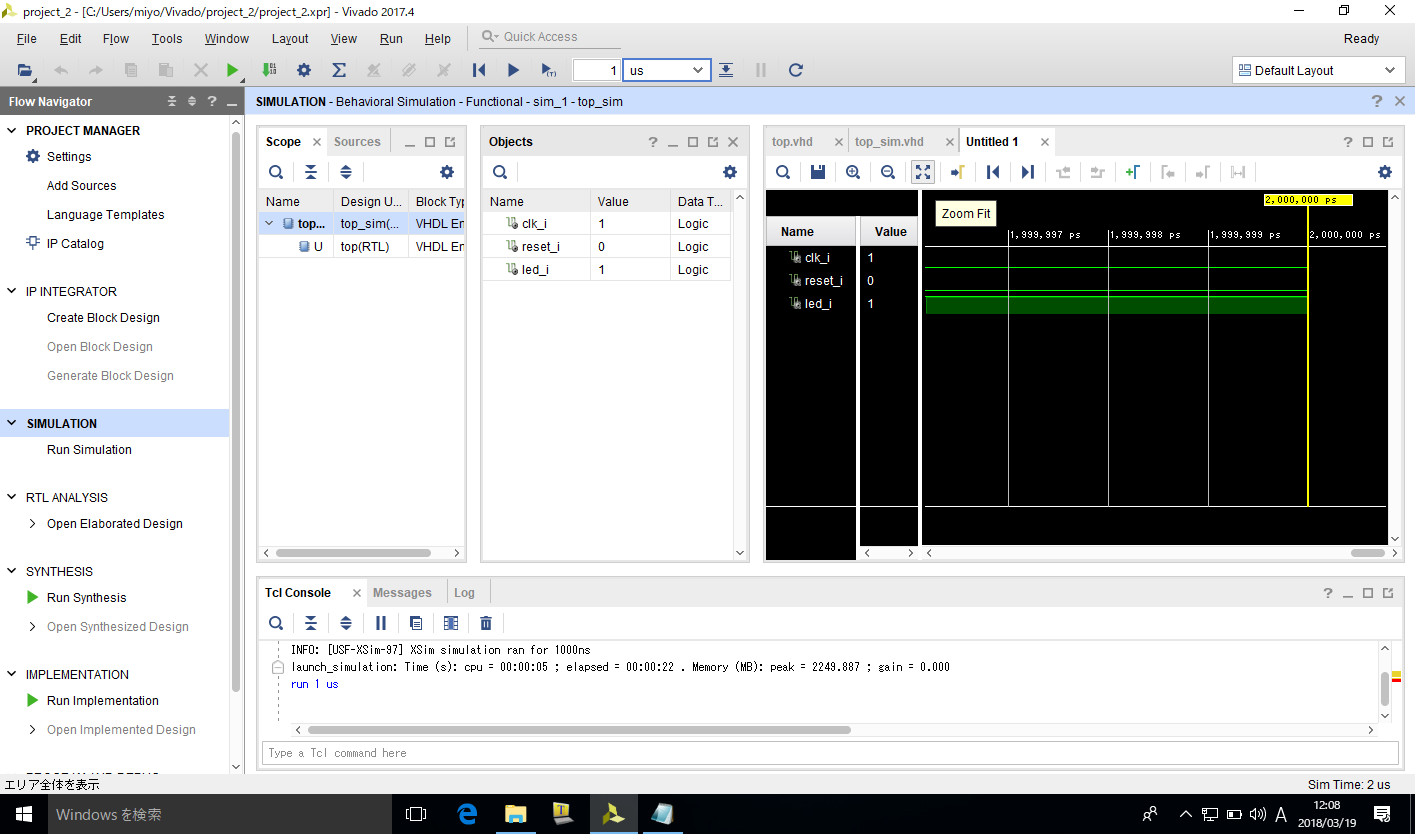
\includegraphics[width=.8\textwidth]{chapter04_figures/VirtualBox_Windows10_19_03_2018_12_08_05.png}
  \end{center}
  \caption{指定した時間のシミュレーションが終了}
 \end{figure}

 \begin{figure}[H]
  \begin{center}
   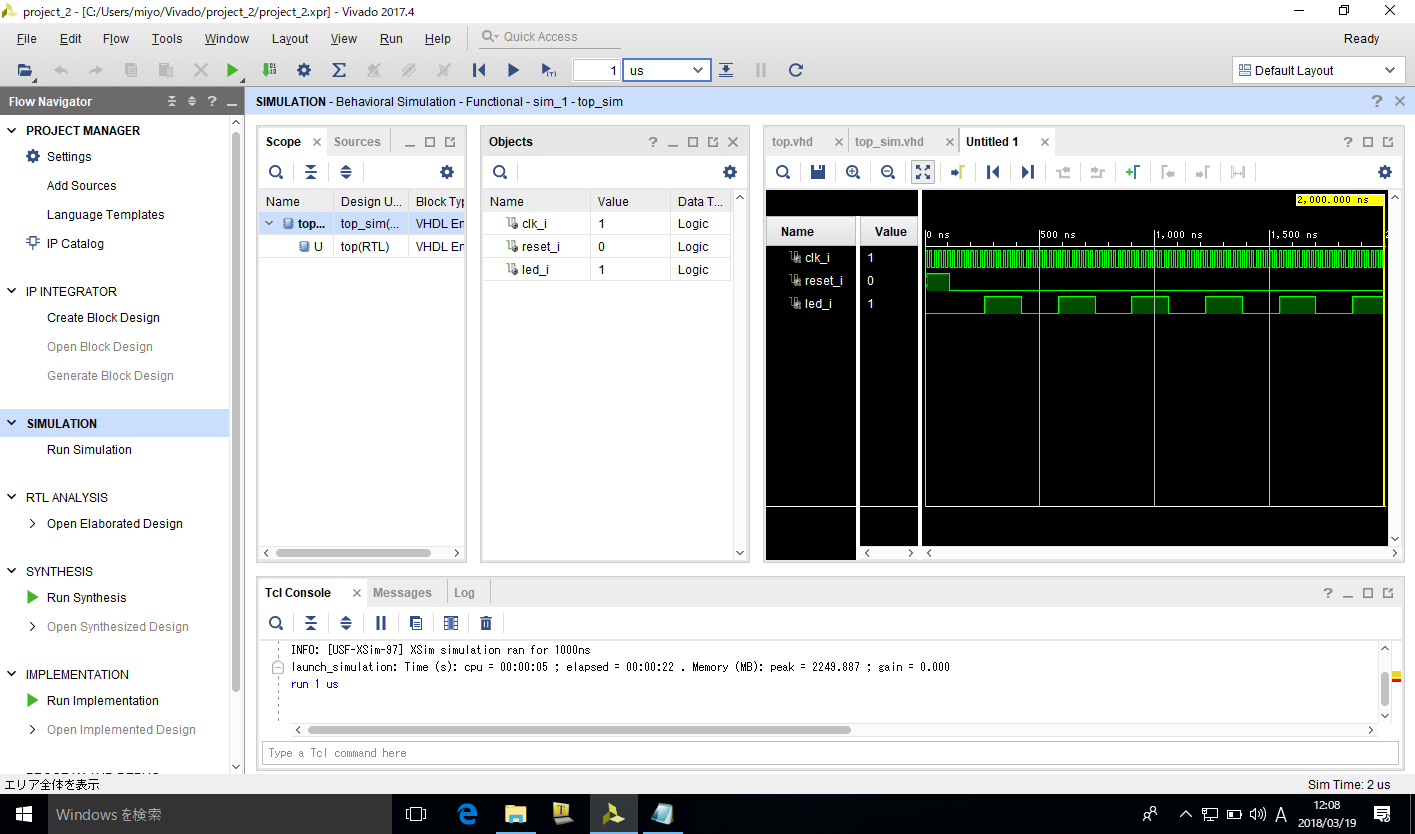
\includegraphics[width=.8\textwidth]{chapter04_figures/VirtualBox_Windows10_19_03_2018_12_08_09.png}
  \end{center}
  \caption{波形表示画面に全シミュレーション結果を表示(FIT)させたところ}
 \end{figure}

 \begin{figure}[H]
  \begin{center}
   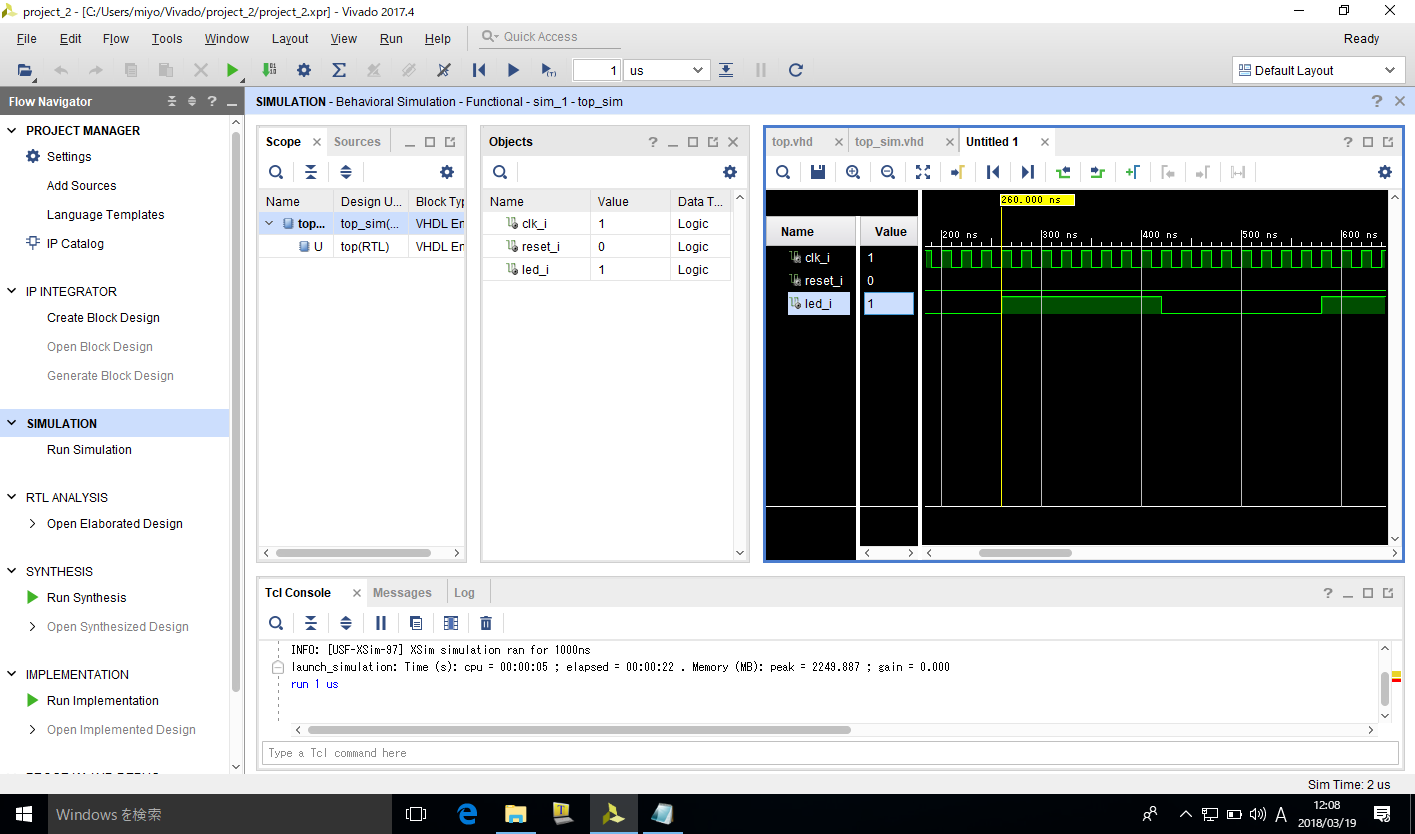
\includegraphics[width=.8\textwidth]{chapter04_figures/VirtualBox_Windows10_19_03_2018_12_08_29.png}
  \end{center}
  \caption{一部分を拡大した様子.3bit目をledに接続しているため8クロック毎にledがON/OFFしている様子がみてとれる}
 \end{figure}

 \begin{figure}[H]
  \begin{center}
   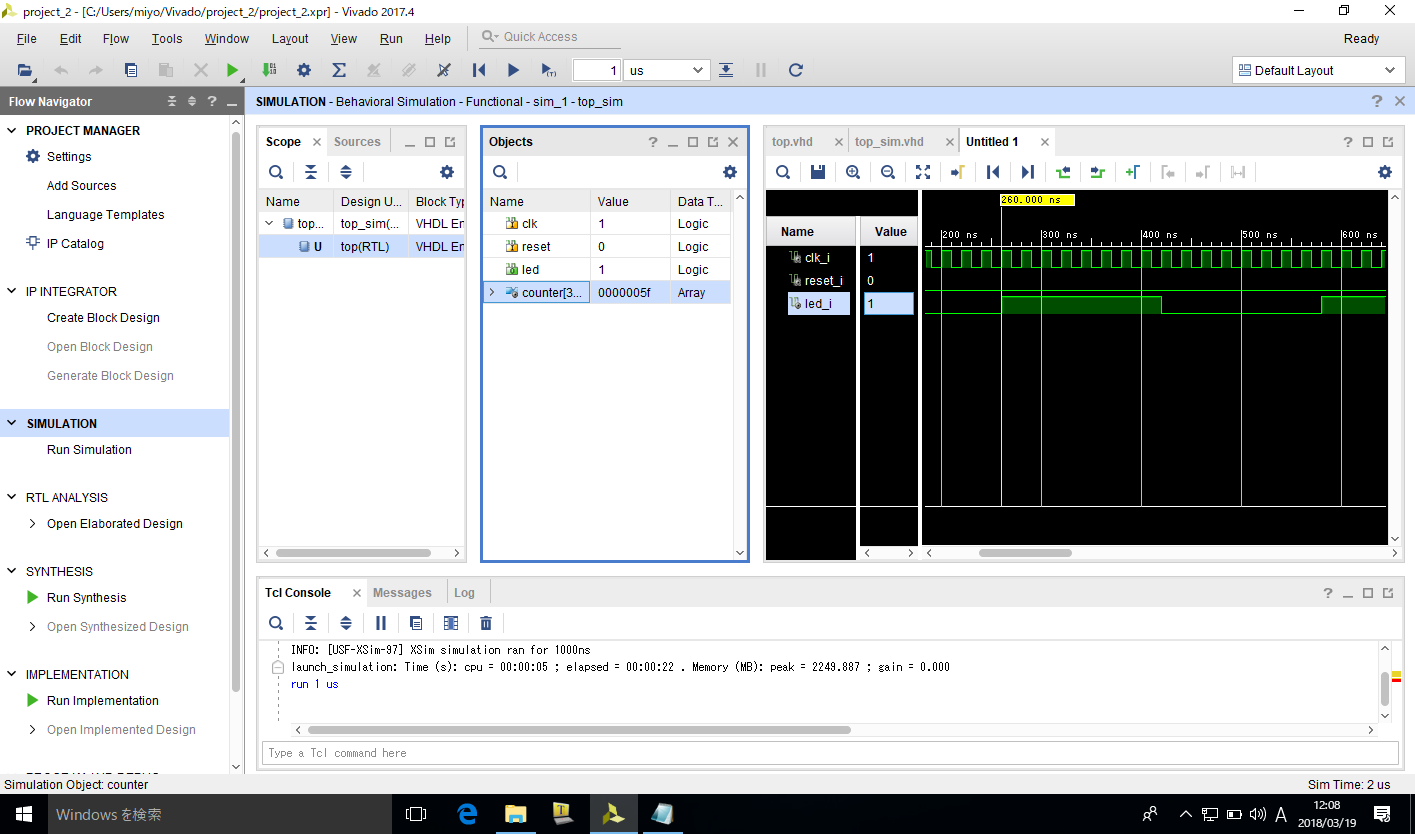
\includegraphics[width=.8\textwidth]{chapter04_figures/VirtualBox_Windows10_19_03_2018_12_08_38.png}
  \end{center}
  \caption{内部モジュール(今回でいうとtopの中身を確認することもできる)}
 \end{figure}

 \begin{figure}[H]
  \begin{center}
   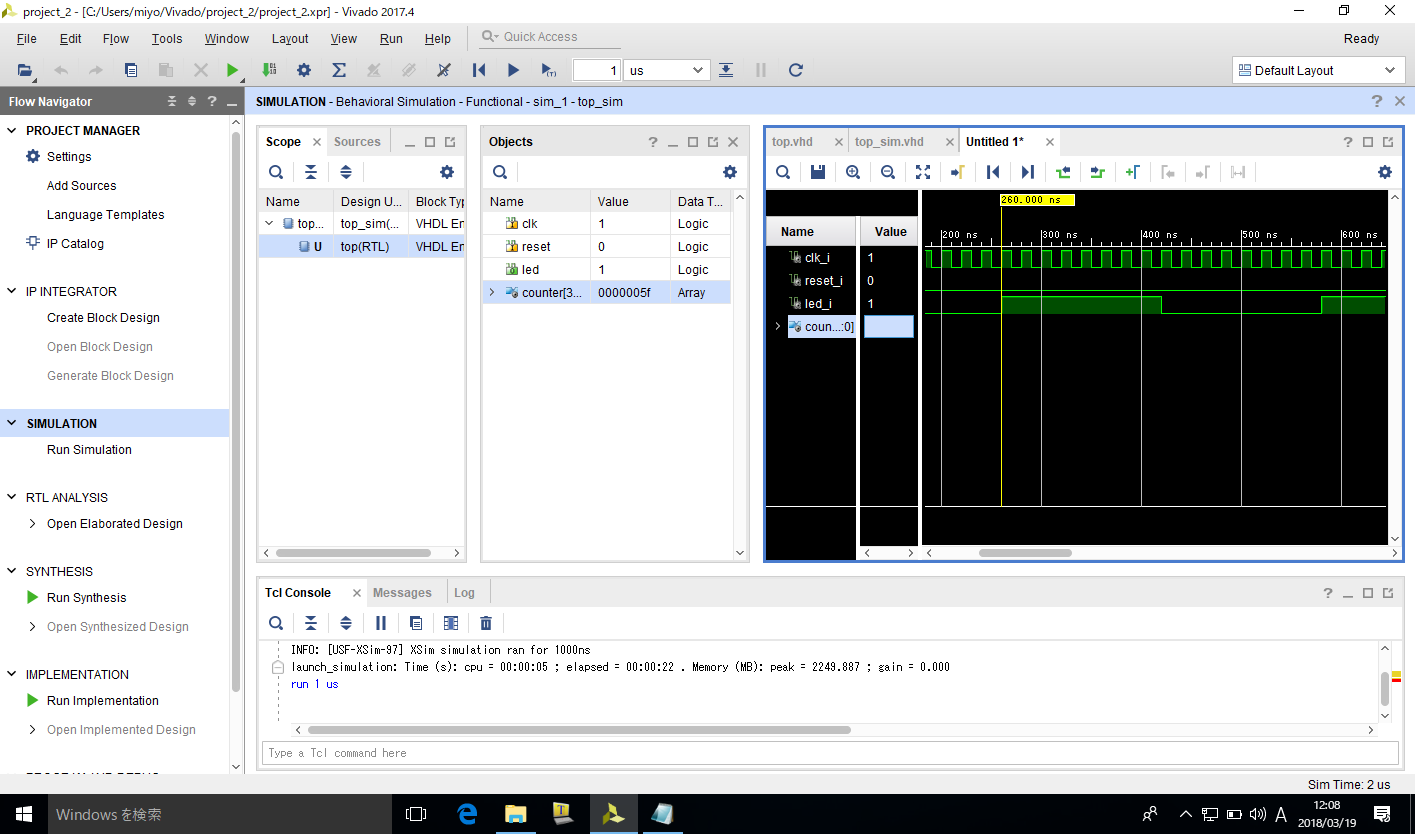
\includegraphics[width=.8\textwidth]{chapter04_figures/VirtualBox_Windows10_19_03_2018_12_08_48.png}
  \end{center}
  \caption{topモジュールのcounterを波形表示画面に追加.ただし,内部の値の多くは非表示状態では保存されていないので,そのままでは値の変化を確認できない}
 \end{figure}

 \begin{figure}[H]
  \begin{center}
   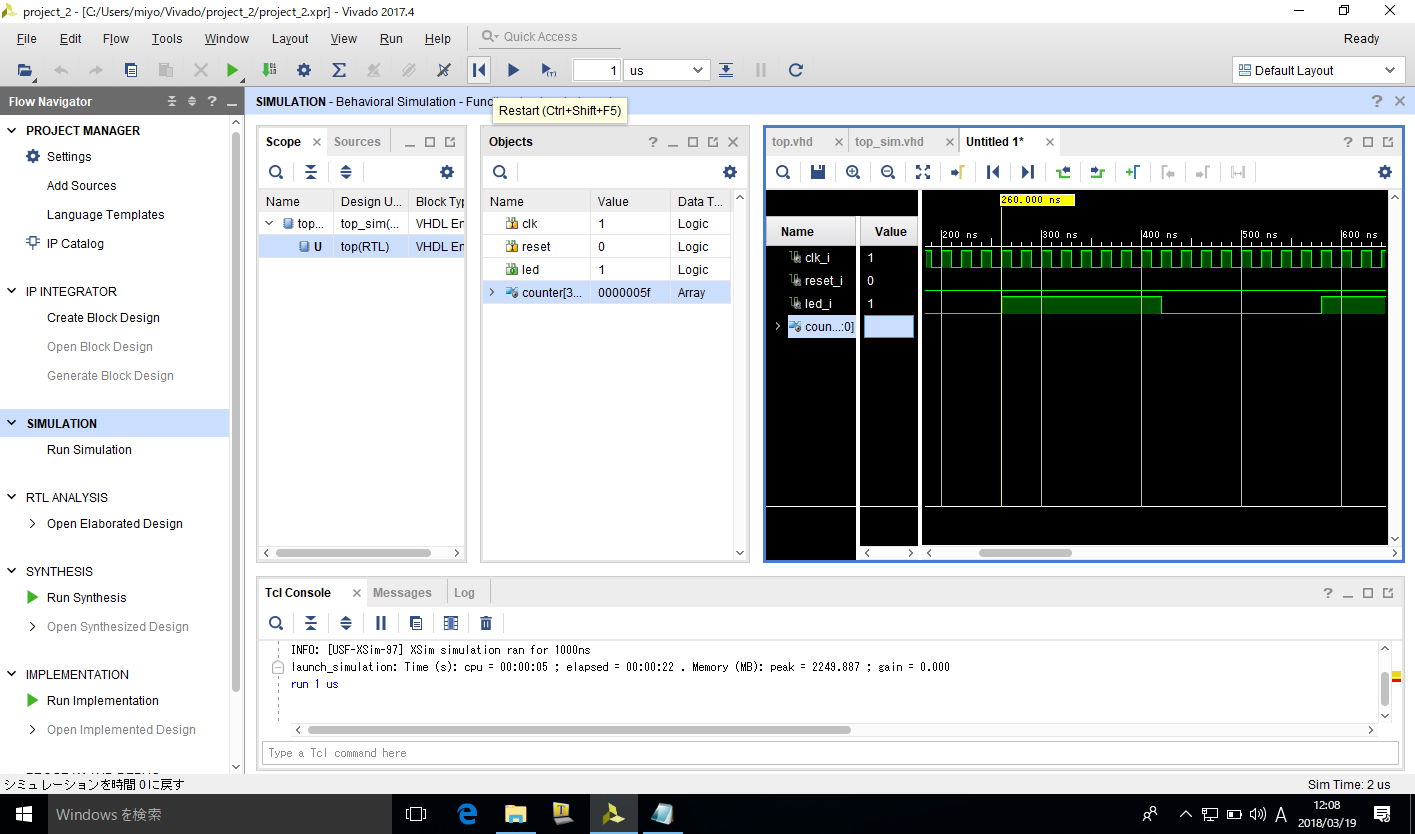
\includegraphics[width=.8\textwidth]{chapter04_figures/VirtualBox_Windows10_19_03_2018_12_08_52.png}
  \end{center}
  \caption{シミュレーションを一度リセット}
 \end{figure}

 \begin{figure}[H]
  \begin{center}
   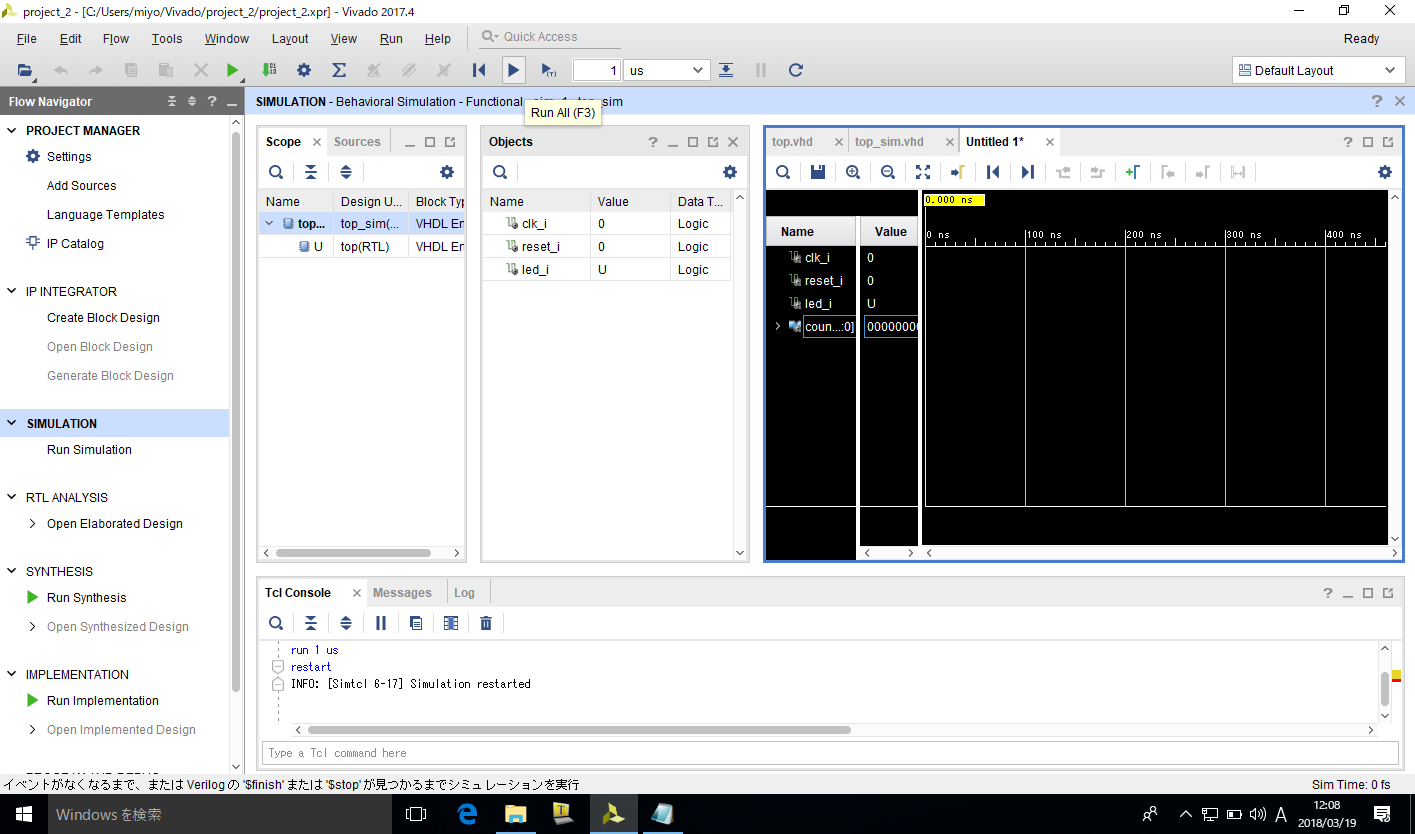
\includegraphics[width=.8\textwidth]{chapter04_figures/VirtualBox_Windows10_19_03_2018_12_08_58.png}
  \end{center}
  \caption{再度シミュレーション.今度は時間指定なくシミューレションしてみる}
 \end{figure}

 \begin{figure}[H]
  \begin{center}
   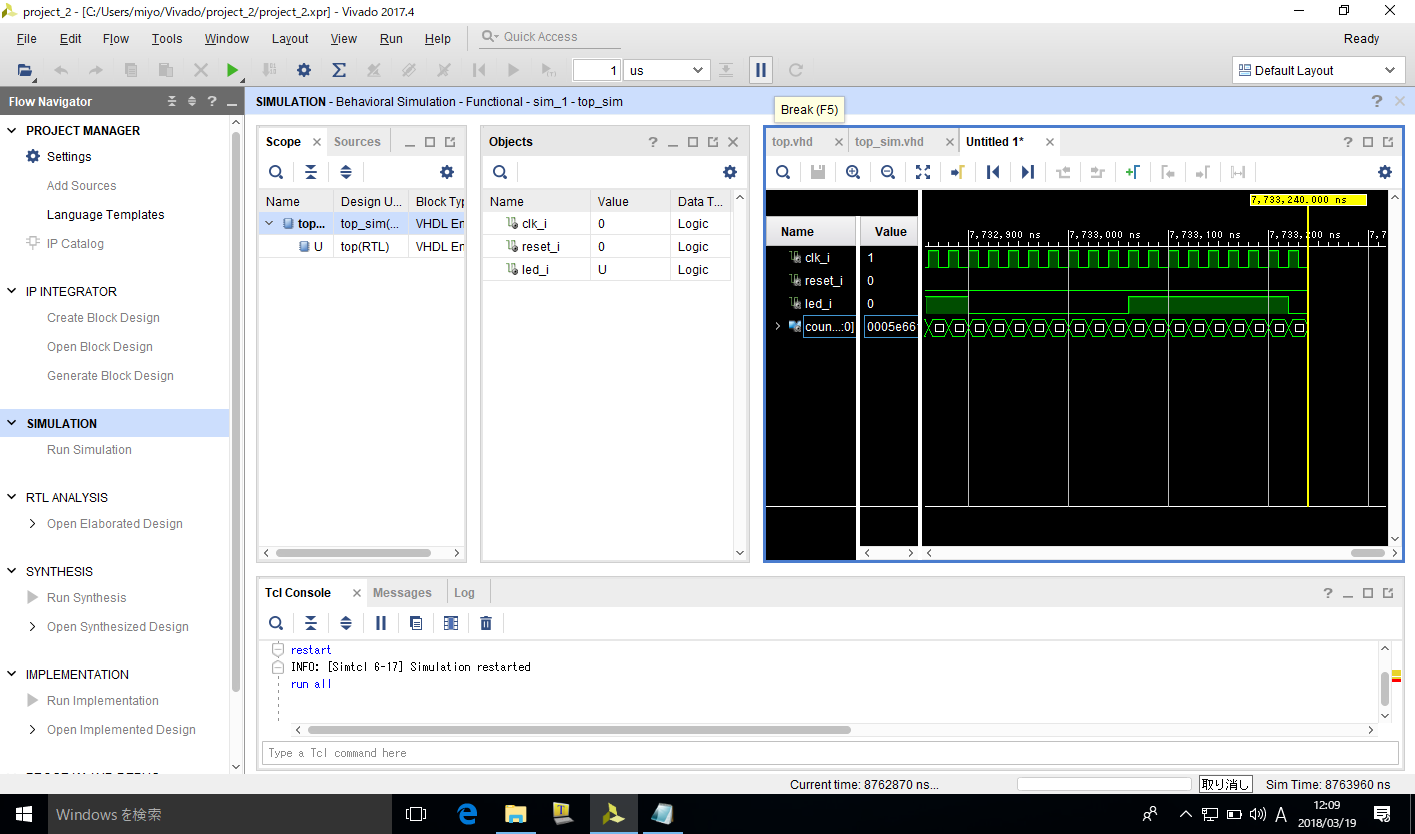
\includegraphics[width=.8\textwidth]{chapter04_figures/VirtualBox_Windows10_19_03_2018_12_09_04.png}
  \end{center}
  \caption{いつまでも終わらないので一時停止アイコンでシミュレーションをストップ}
 \end{figure}

 \begin{figure}[H]
  \begin{center}
   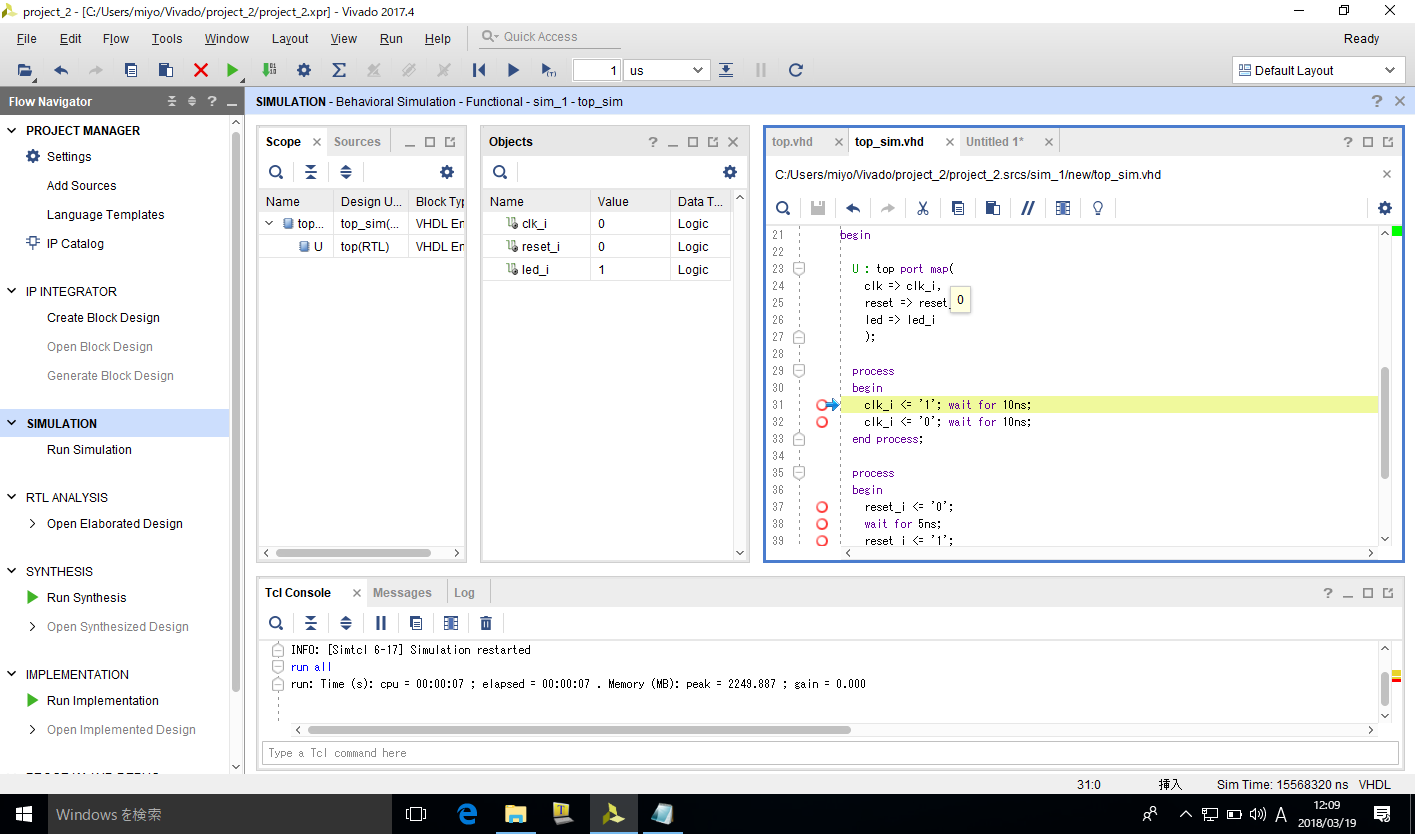
\includegraphics[width=.8\textwidth]{chapter04_figures/VirtualBox_Windows10_19_03_2018_12_09_10.png}
  \end{center}
  \caption{ストップした箇所のソースコードが表示される}
 \end{figure}

 \begin{figure}[H]
  \begin{center}
   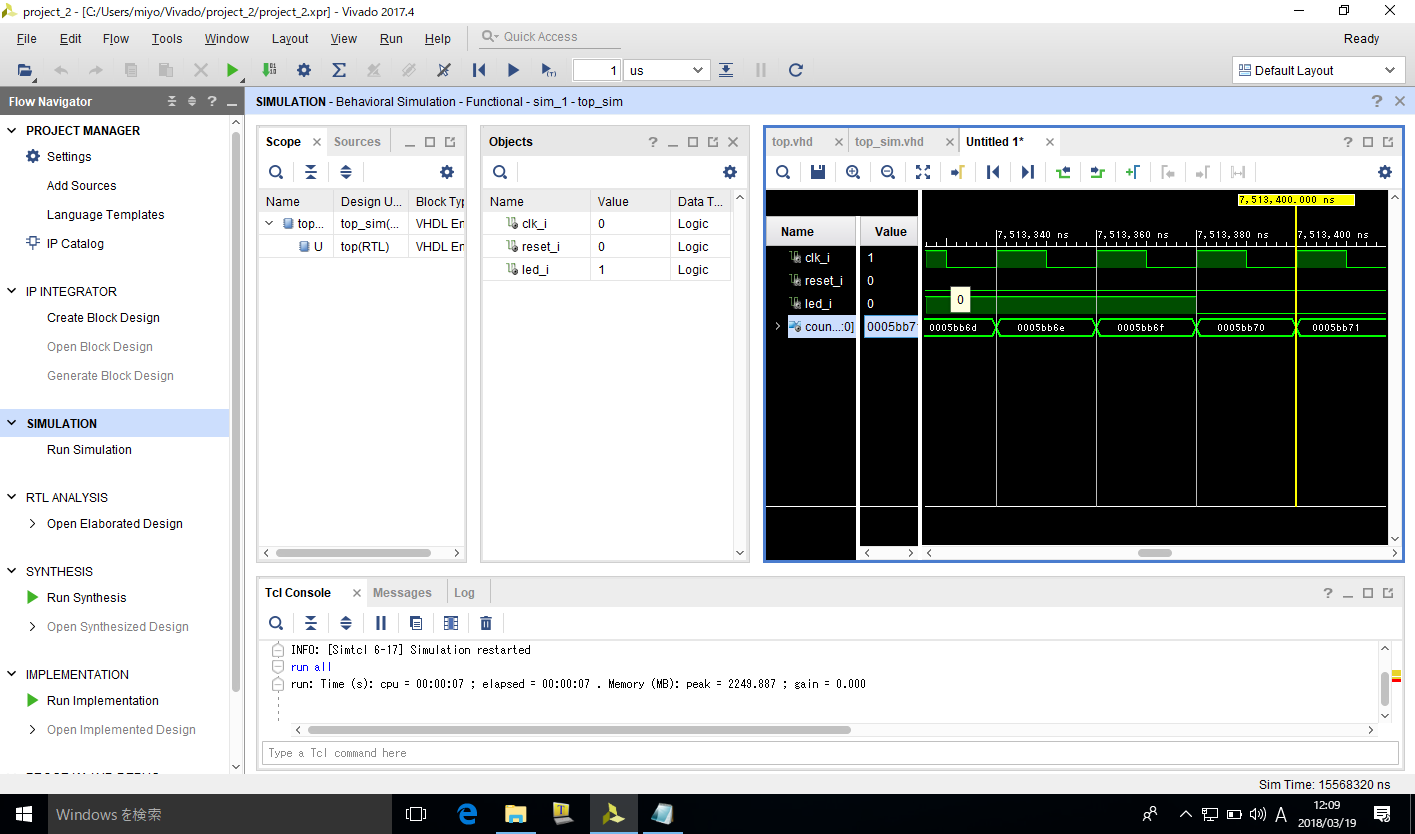
\includegraphics[width=.8\textwidth]{chapter04_figures/VirtualBox_Windows10_19_03_2018_12_09_39.png}
  \end{center}
  \caption{波形を確認してみると,内部のcounterがclkにあわせてインクリメントしていること,counterの3bit目がledの'0'/'1'と同じであることが確認できる}
 \end{figure}

\section{課題}
\begin{enumerate}
 \item 点滅の間隔を変えてみたときの様子をシミュレーションしてみよう
 \item resetを適当なタイミングで変化させてみて,counterやledの振る舞いを観察してみよう
\end{enumerate}

\end{document}
